\documentclass[a4j]{jarticle}
\usepackage[dvipdfmx]{graphicx}
\usepackage{amssymb}
\usepackage{subfigure}

\begin{document}
\begin{center}
{\large 現状得られているデータとその結果のご報告}
\end{center}
\begin{description}
\item[データ1] \\
ping による応答遅延の計測を 10 ミリ秒間隔で計 10 回行う操作を 5 秒毎に実行した.また,計測期間は計 1 時間とした.ping コマンドの実行時刻が早いものから順に $t = 1,2,\ldots$ とし,$t$ を横軸に,縦軸にはそれに対応する ping 応答遅延時間 [ms] をとった結果を図 \ref{data1-1} から図 \ref{data1-2} に示す.この図では,縦軸に垂直な黒線で ping の実行時刻に応じた組分けをしており,組内の ping の実行間隔は 10 ミリ秒,組間の先頭の ping の実行間隔が 5 秒となるようにしている.
\begin{figure}[tb]
\begin{center}
\subfigure[$0 \sim 1$ 分後]{
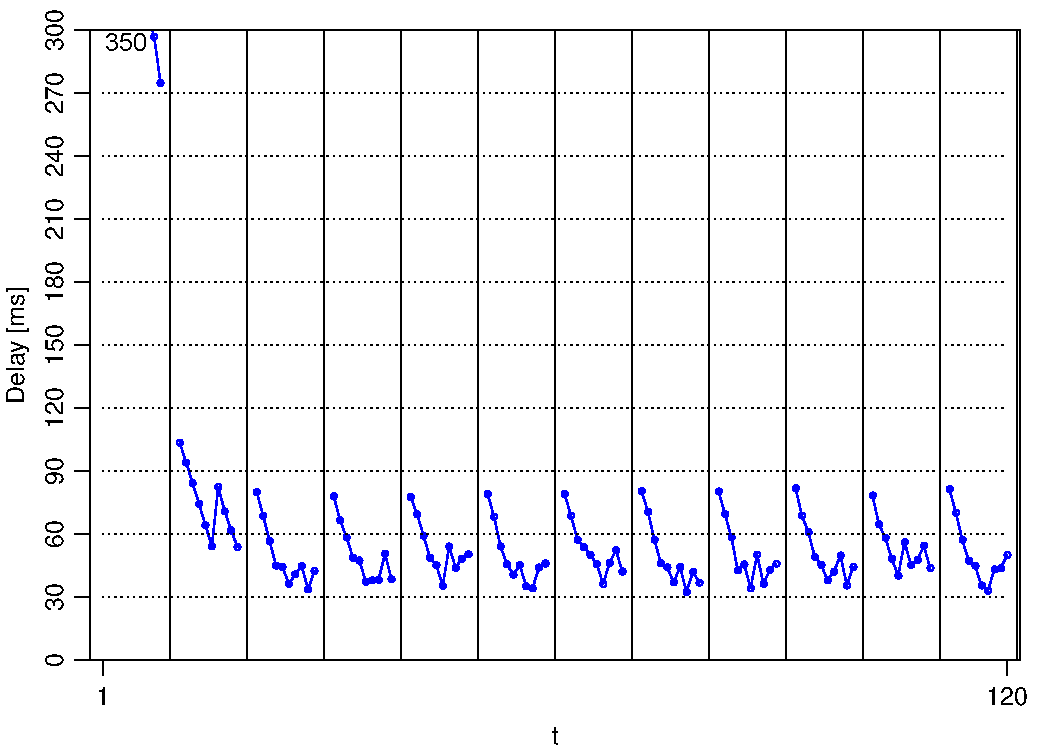
\includegraphics[width=0.33\hsize]{0-1.pdf}
}~
\subfigure[$1 \sim 2$ 分後]{
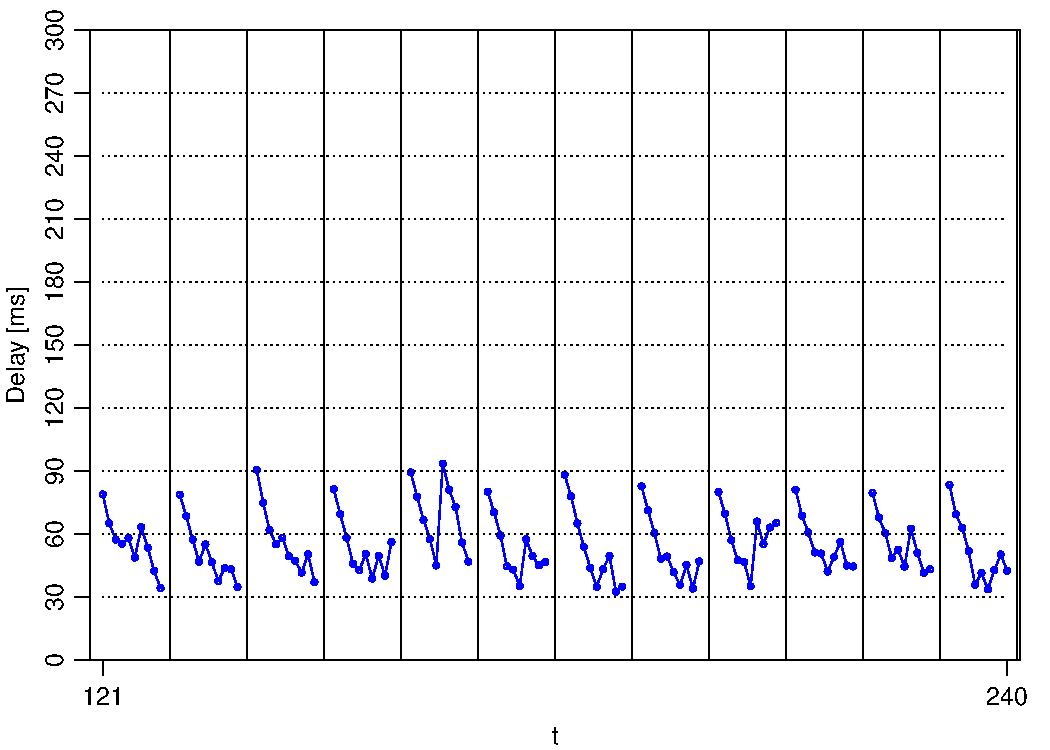
\includegraphics[width=0.33\hsize]{1-2.pdf}
}~
\subfigure[$2 \sim 3$ 分後]{
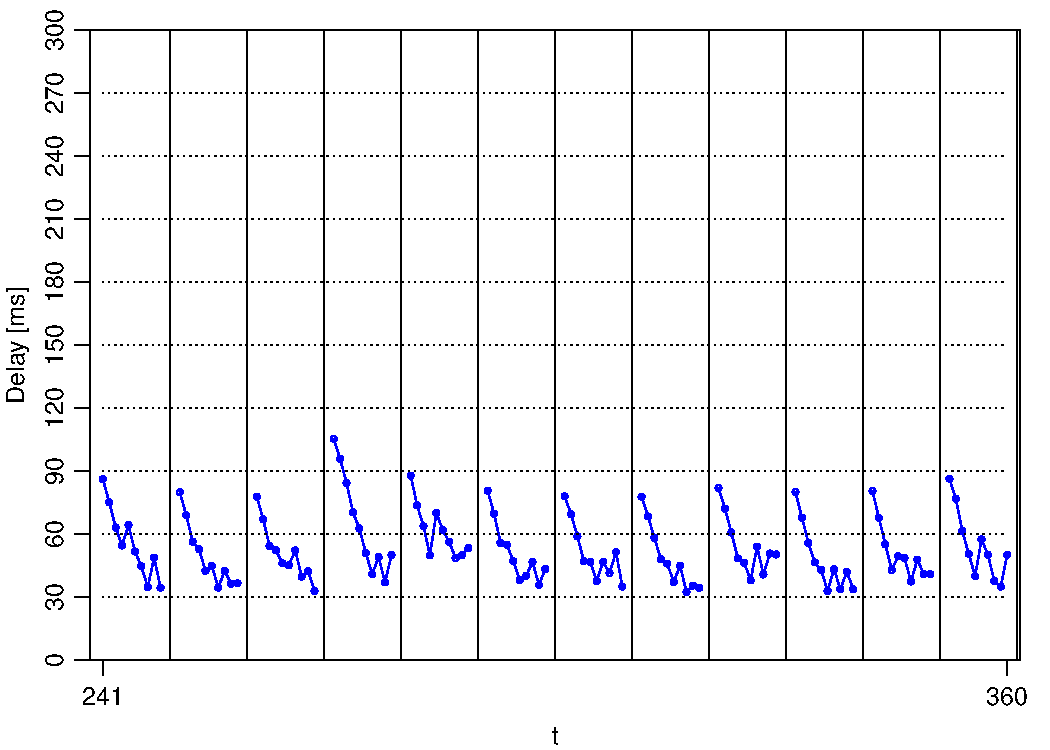
\includegraphics[width=0.33\hsize]{2-3.pdf}
}\\

\subfigure[$3 \sim 4$ 分後]{
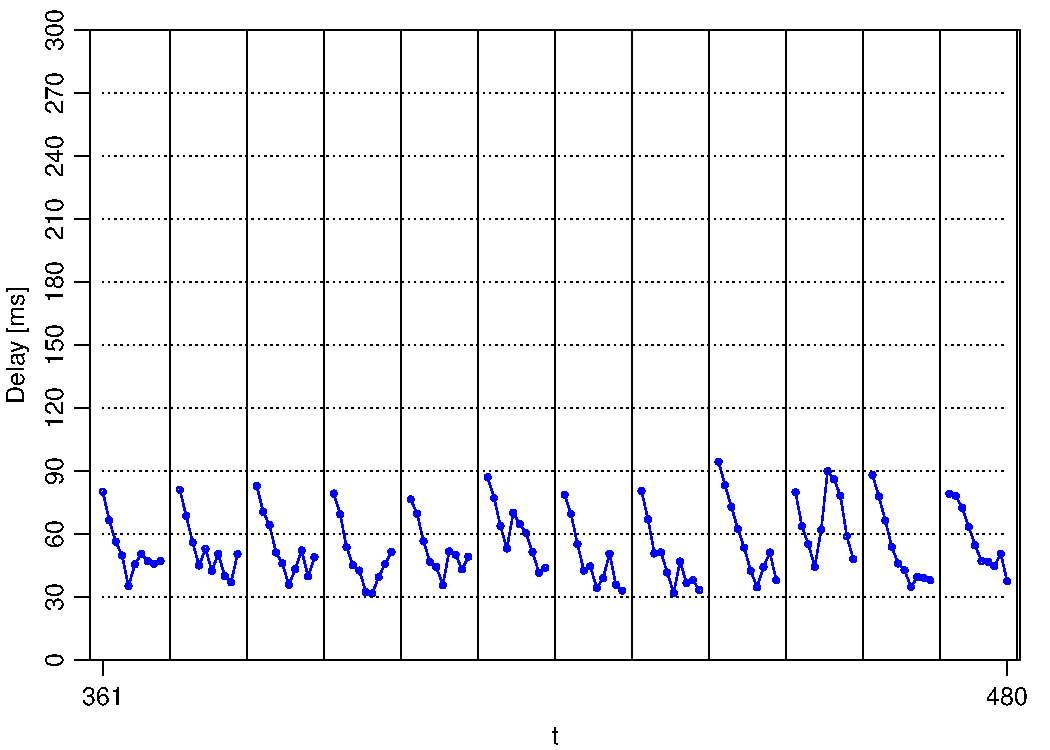
\includegraphics[width=0.33\hsize]{3-4.pdf}
}~
\subfigure[$4 \sim 5$ 分後]{
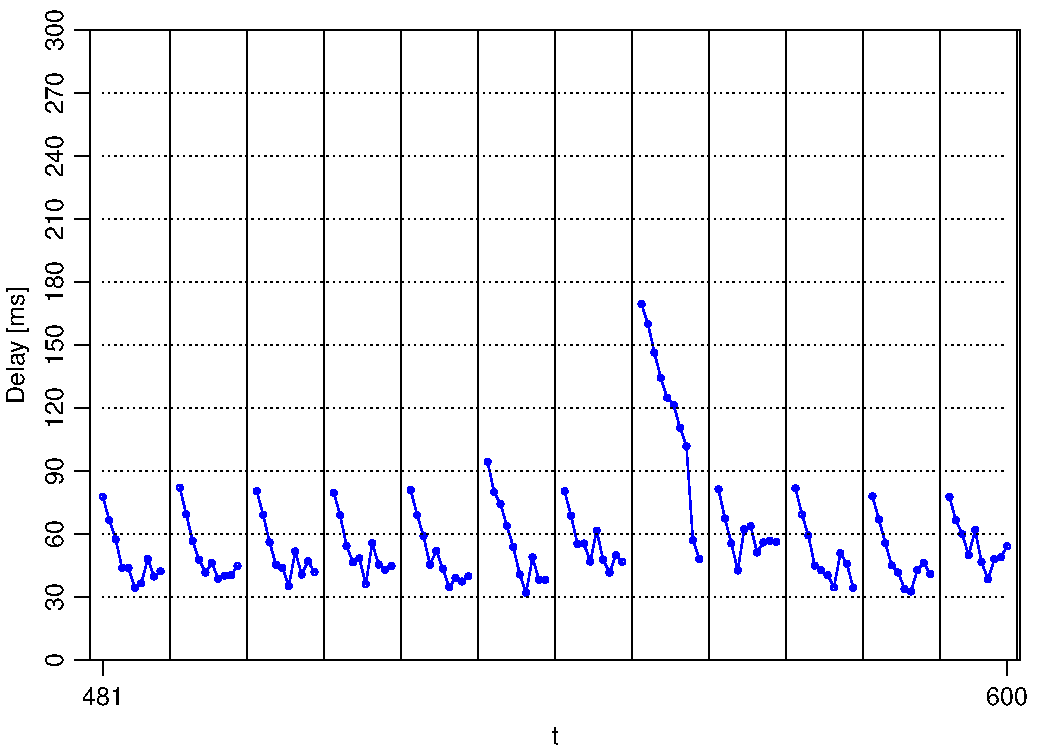
\includegraphics[width=0.33\hsize]{4-5.pdf}
}~
\subfigure[$5 \sim 6$ 分後]{
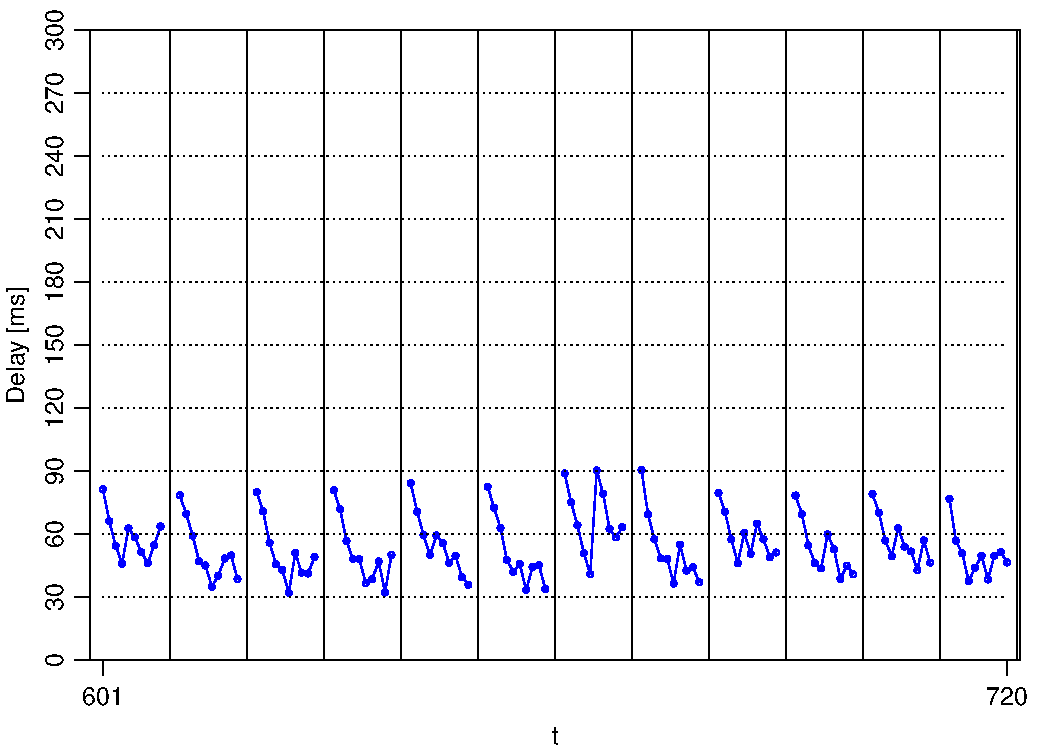
\includegraphics[width=0.33\hsize]{5-6.pdf}
}\\

\subfigure[$6 \sim 7$ 分後]{
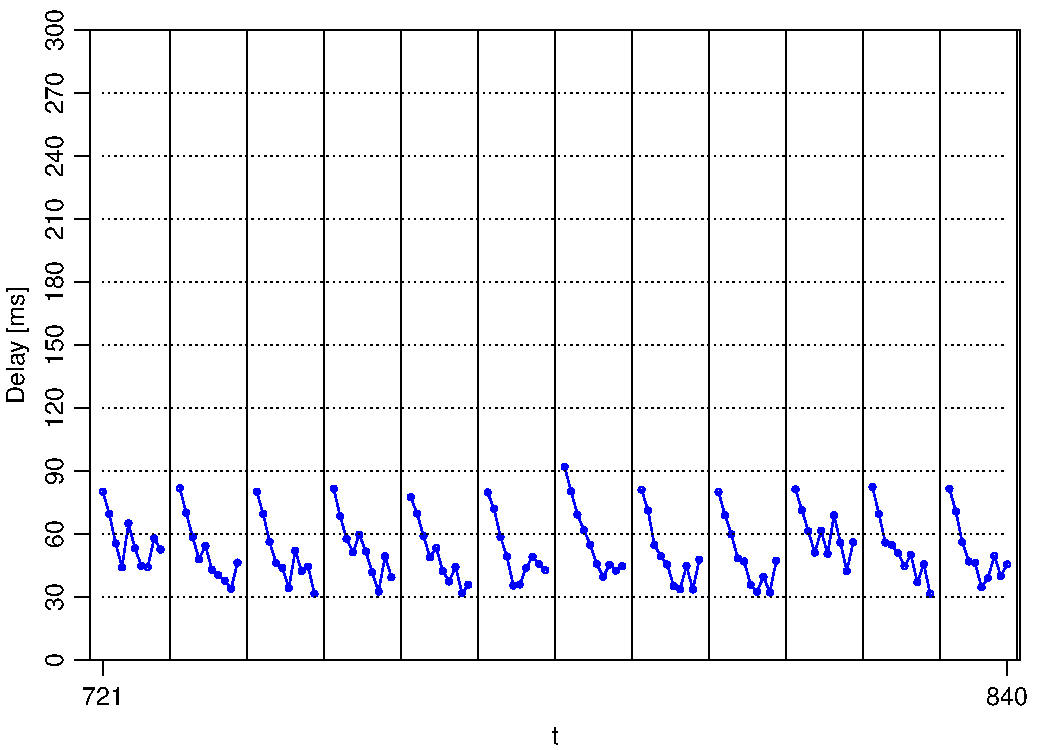
\includegraphics[width=0.33\hsize]{6-7.pdf}
}~
\subfigure[$7 \sim 8$ 分後]{
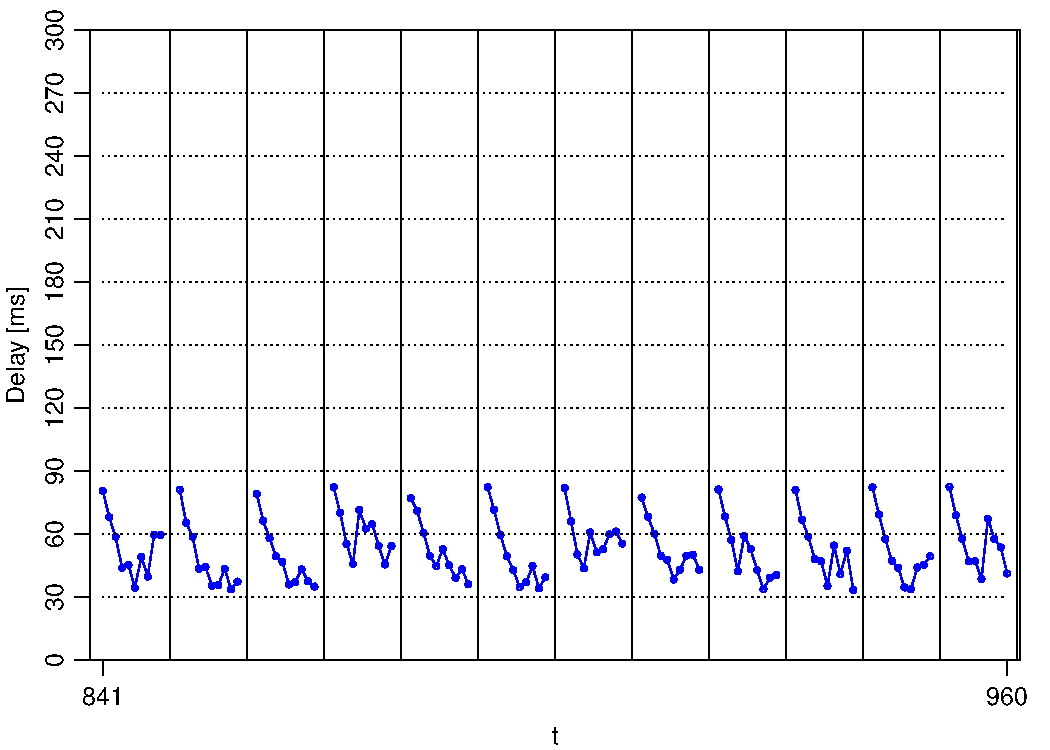
\includegraphics[width=0.33\hsize]{7-8.pdf}
}~
\subfigure[$8 \sim 9$ 分後]{
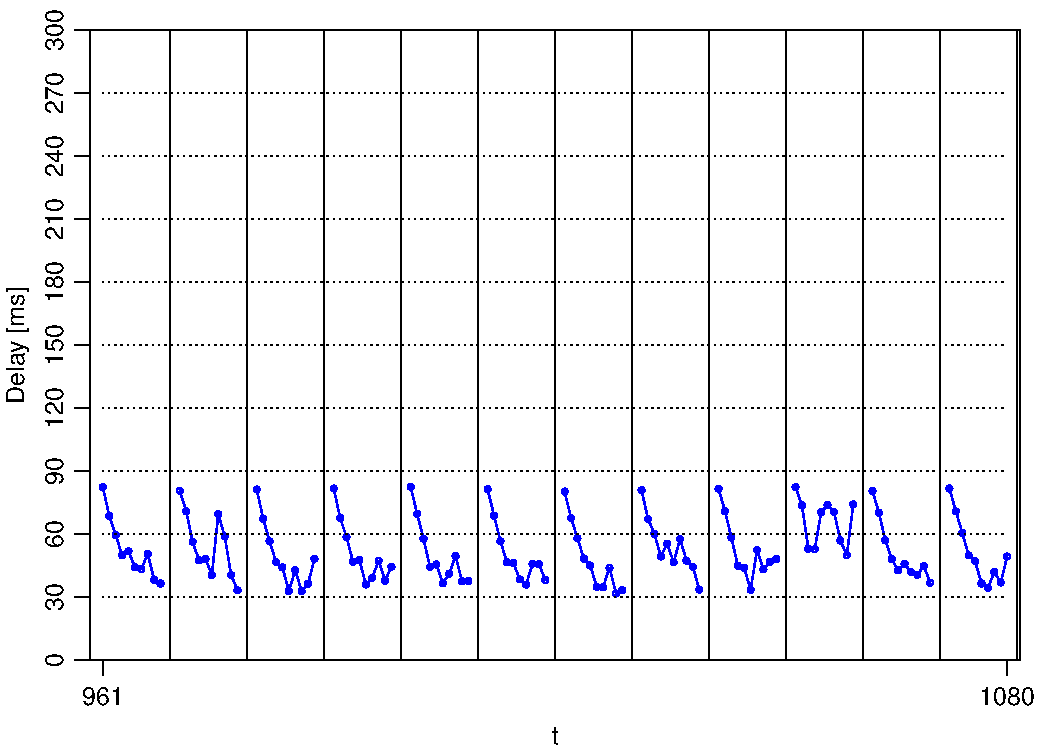
\includegraphics[width=0.33\hsize]{8-9.pdf}
}\\

\subfigure[$9 \sim 10$ 分後]{
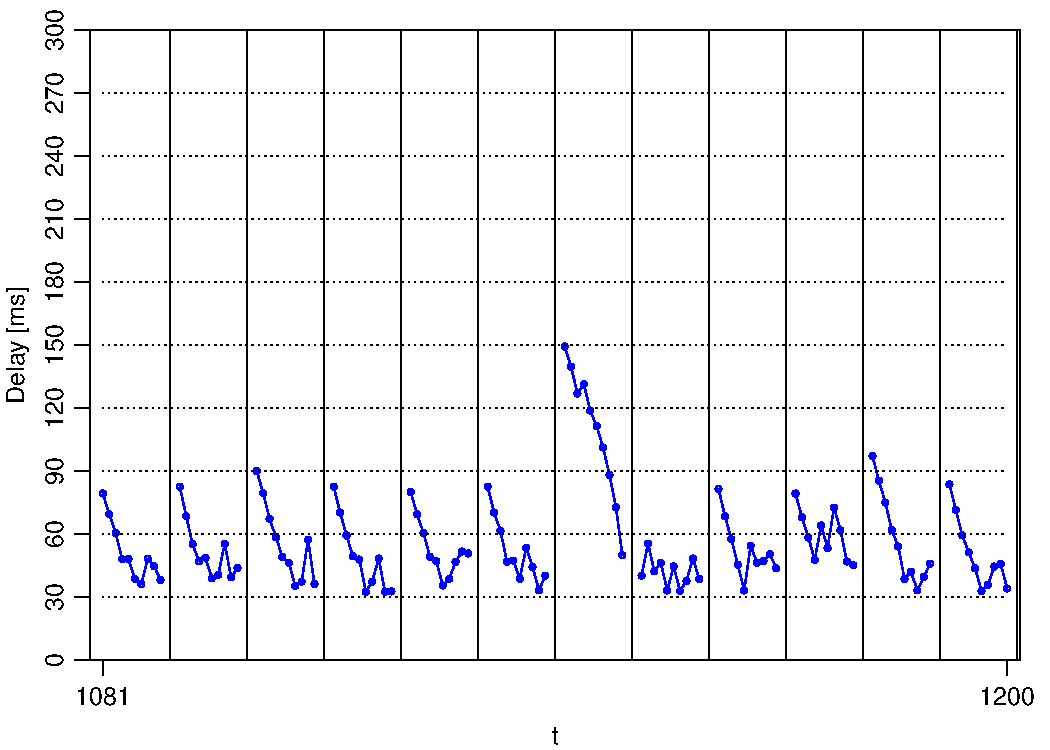
\includegraphics[width=0.33\hsize]{9-10.pdf}
}~
\subfigure[$10 \sim 11$ 分後]{
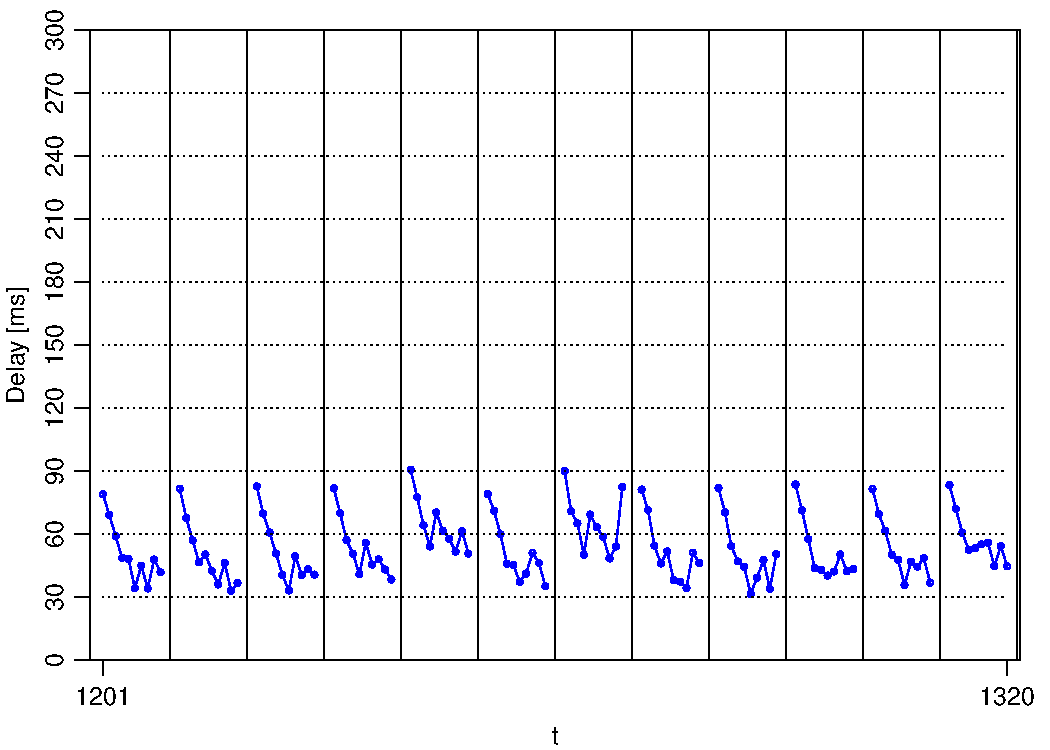
\includegraphics[width=0.33\hsize]{10-11.pdf}
}~
\subfigure[$11 \sim 12$ 分後]{
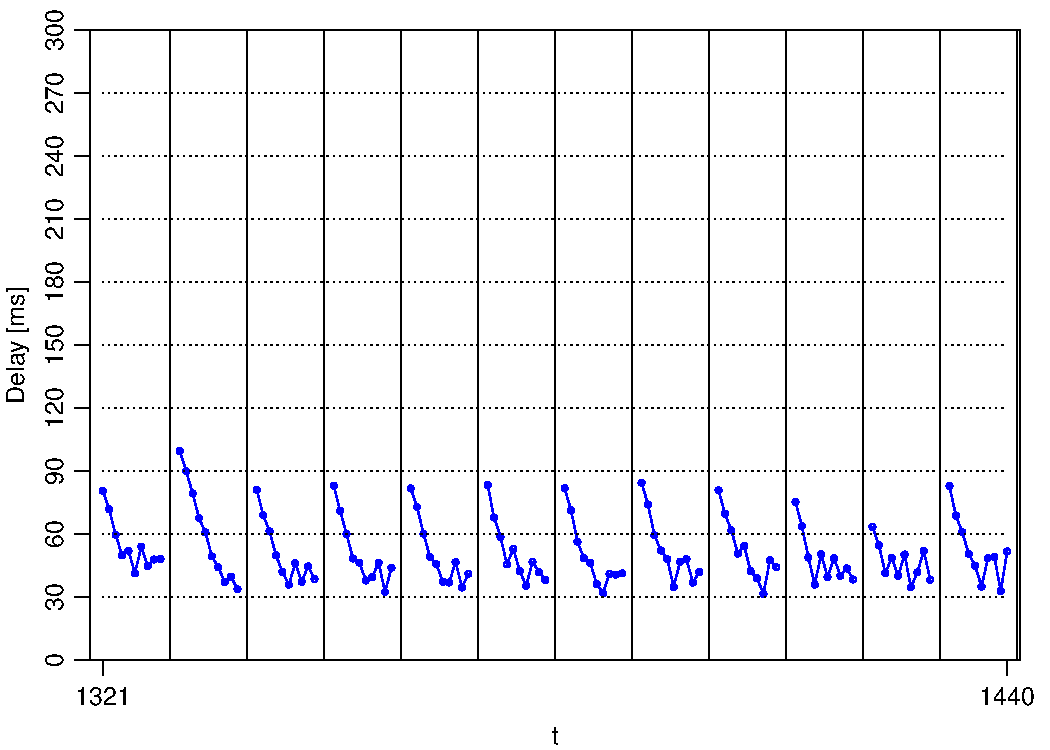
\includegraphics[width=0.33\hsize]{11-12.pdf}
}\\

\subfigure[$12 \sim 13$ 分後]{
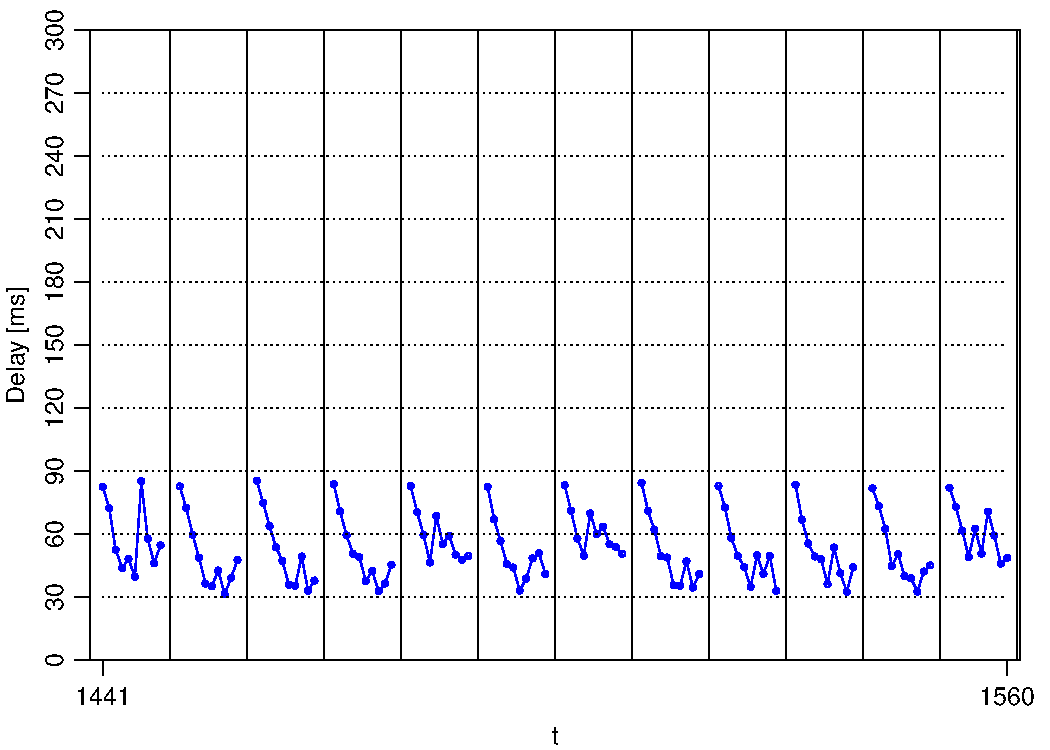
\includegraphics[width=0.33\hsize]{12-13.pdf}
}~
\subfigure[$13 \sim 14$ 分後]{
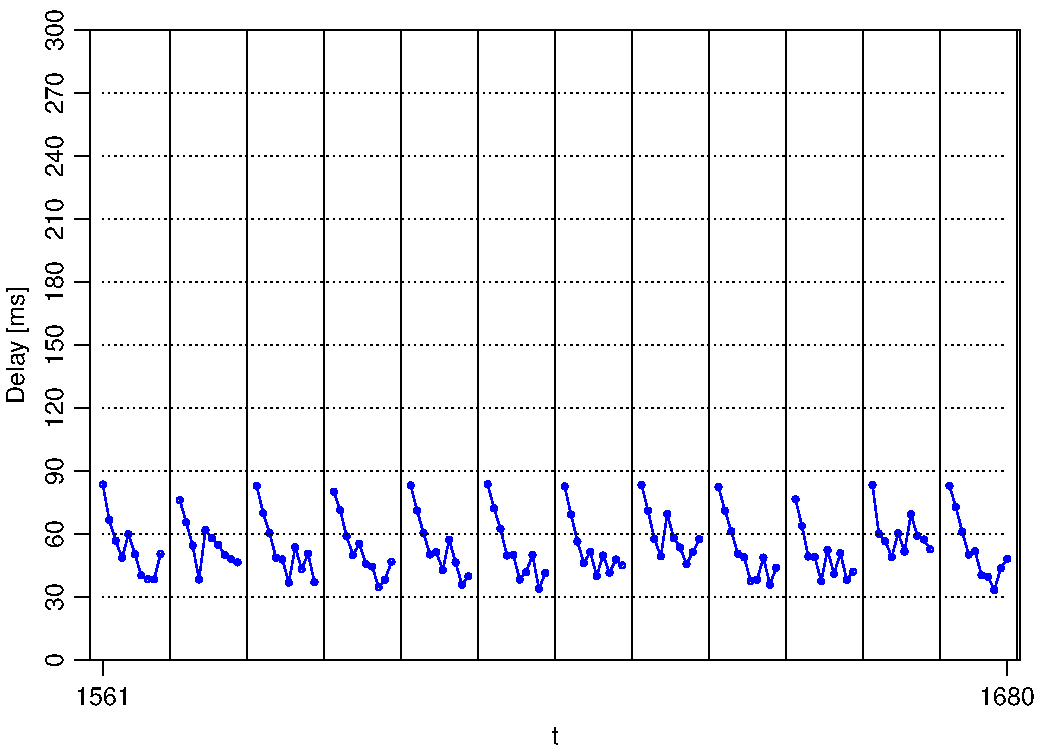
\includegraphics[width=0.33\hsize]{13-14.pdf}
}~
\subfigure[$14 \sim 15$ 分後]{
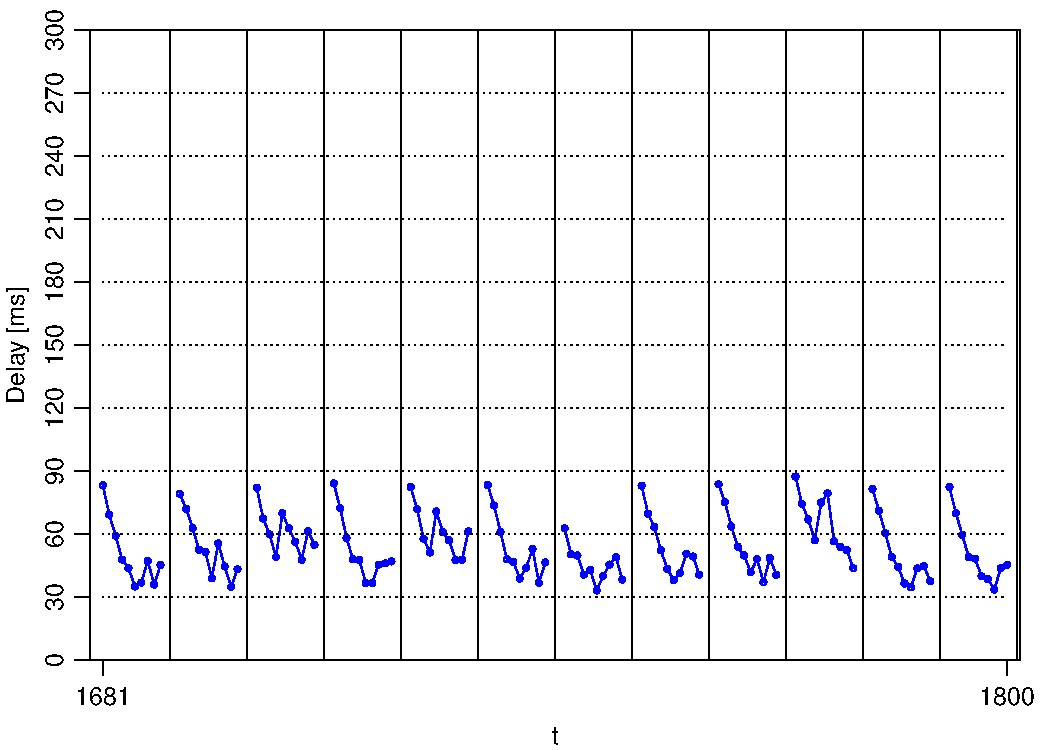
\includegraphics[width=0.33\hsize]{14-15.pdf}
}
\caption{10 ミリ秒間隔で計 10 回の ping 実行を 5 秒毎に行った計測結果(開始から 15 分後まで)}
\label{data1-1}
\end{center}
\end{figure}

\begin{figure}[tb]
\begin{center}
\subfigure[$15 \sim 16$ 分後]{
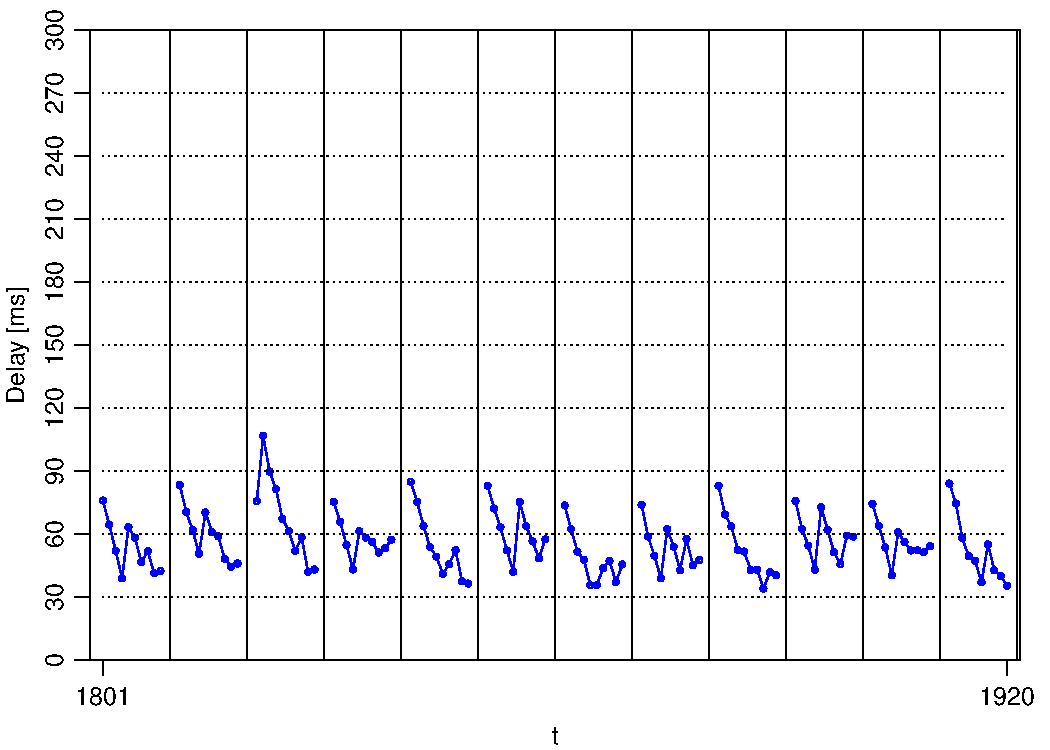
\includegraphics[width=0.33\hsize]{15-16.pdf}
}~
\subfigure[$16 \sim 17$ 分後]{
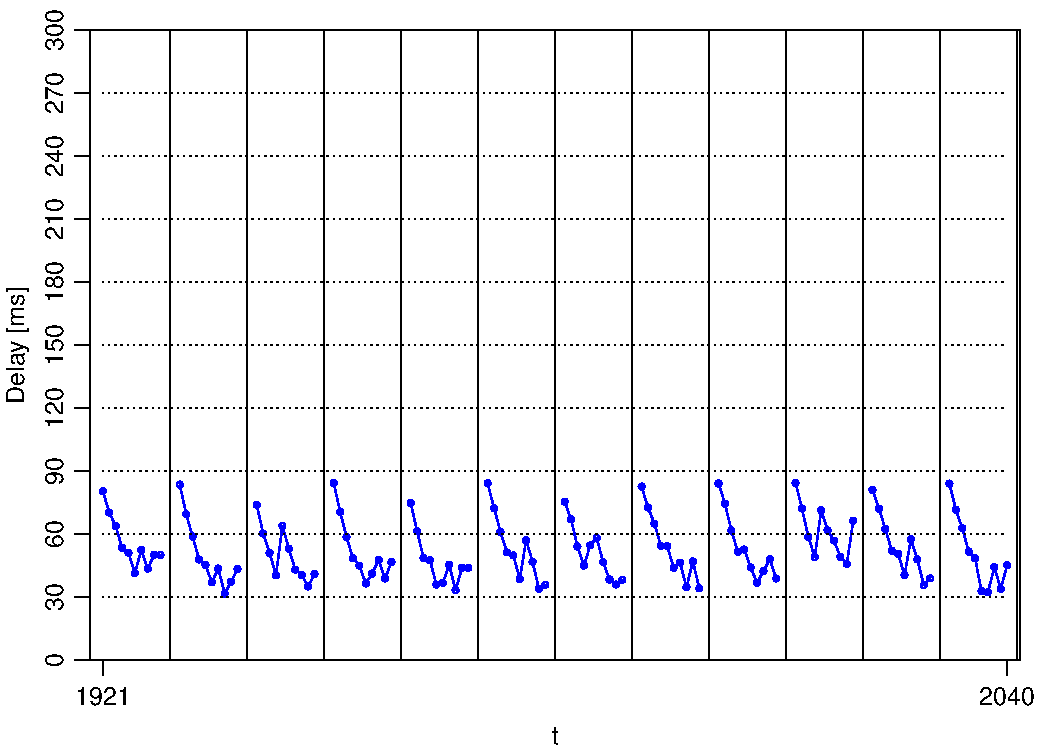
\includegraphics[width=0.33\hsize]{16-17.pdf}
}~
\subfigure[$17 \sim 18$ 分後]{
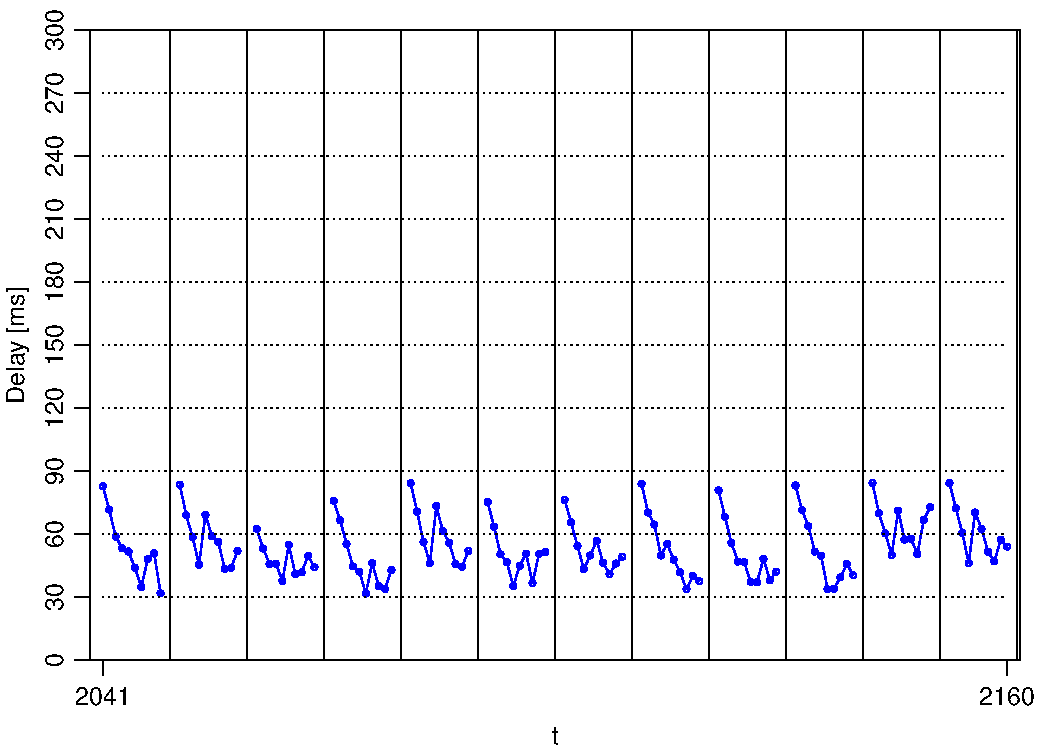
\includegraphics[width=0.33\hsize]{17-18.pdf}
}\\

\subfigure[$18 \sim 19$ 分後]{
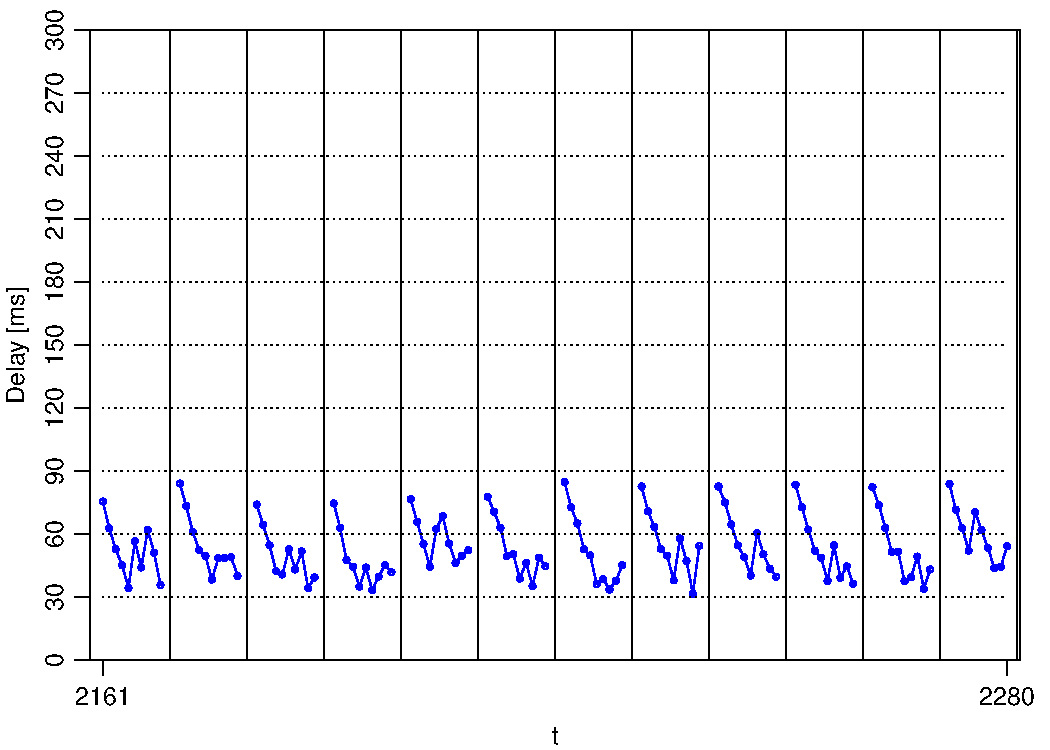
\includegraphics[width=0.33\hsize]{18-19.pdf}
}~
\subfigure[$19 \sim 20$ 分後]{
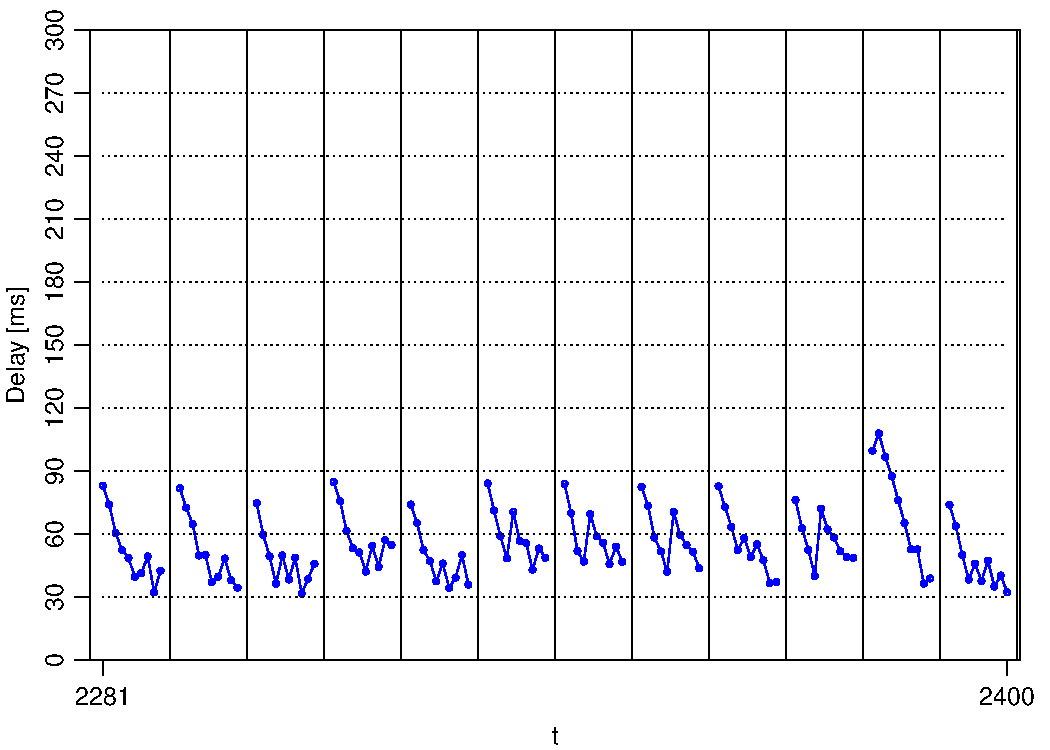
\includegraphics[width=0.33\hsize]{19-20.pdf}
}~
\subfigure[$20 \sim 21$ 分後]{
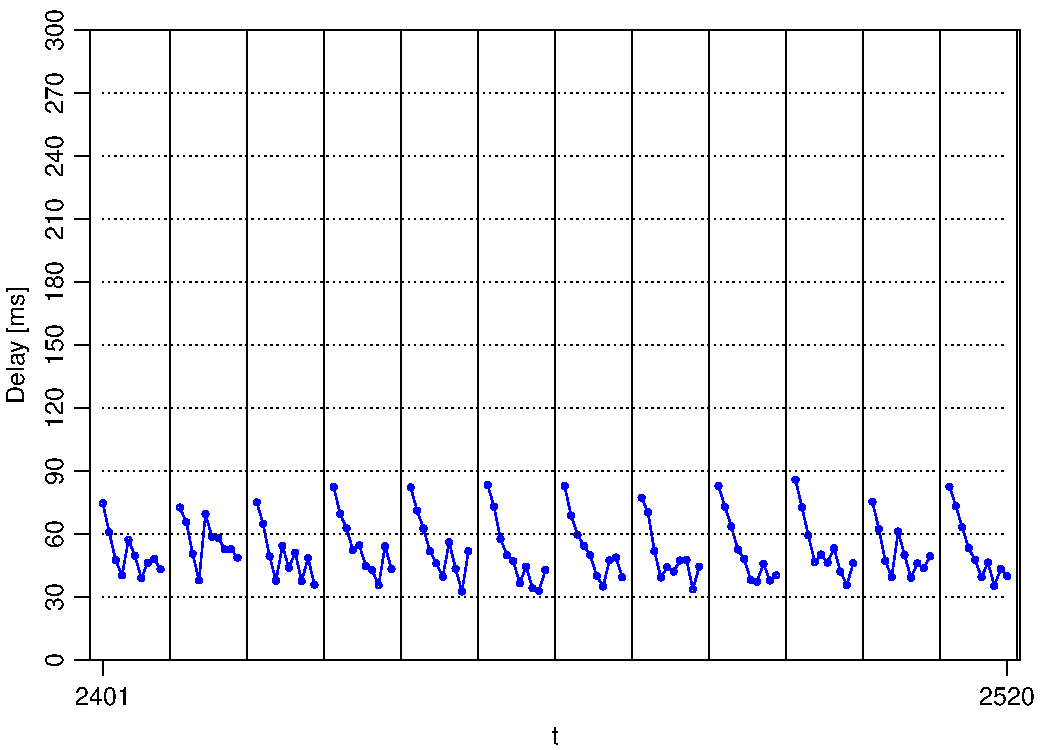
\includegraphics[width=0.33\hsize]{20-21.pdf}
}\\

\subfigure[$21 \sim 22$ 分後]{
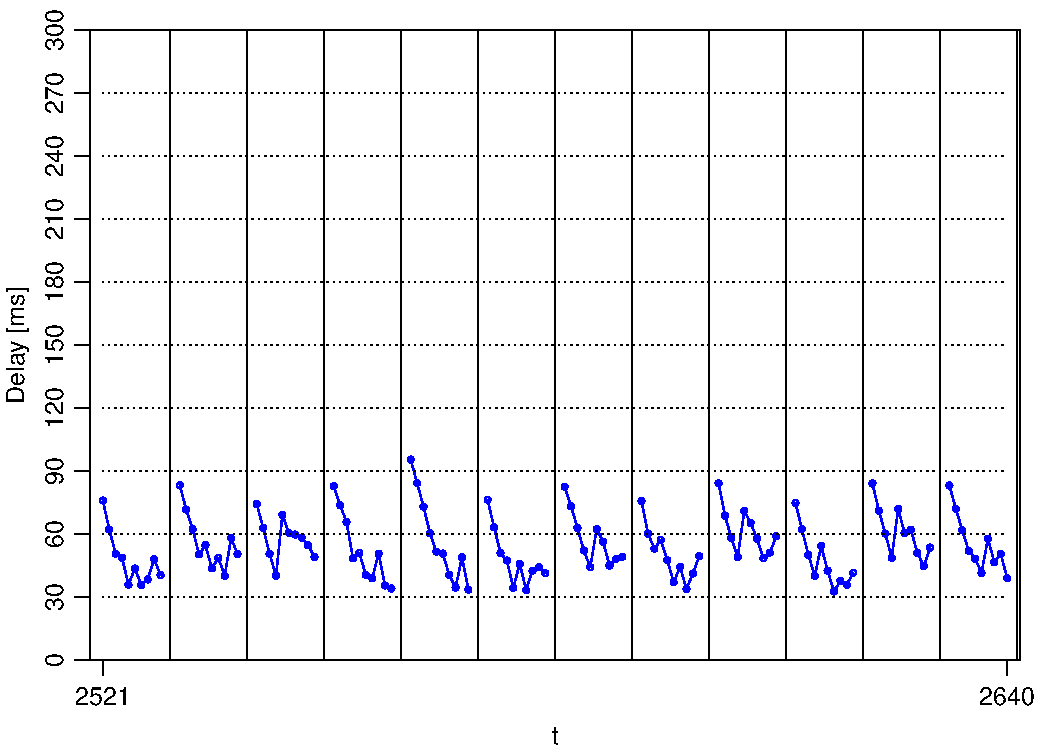
\includegraphics[width=0.33\hsize]{21-22.pdf}
}~
\subfigure[$22 \sim 23$ 分後]{
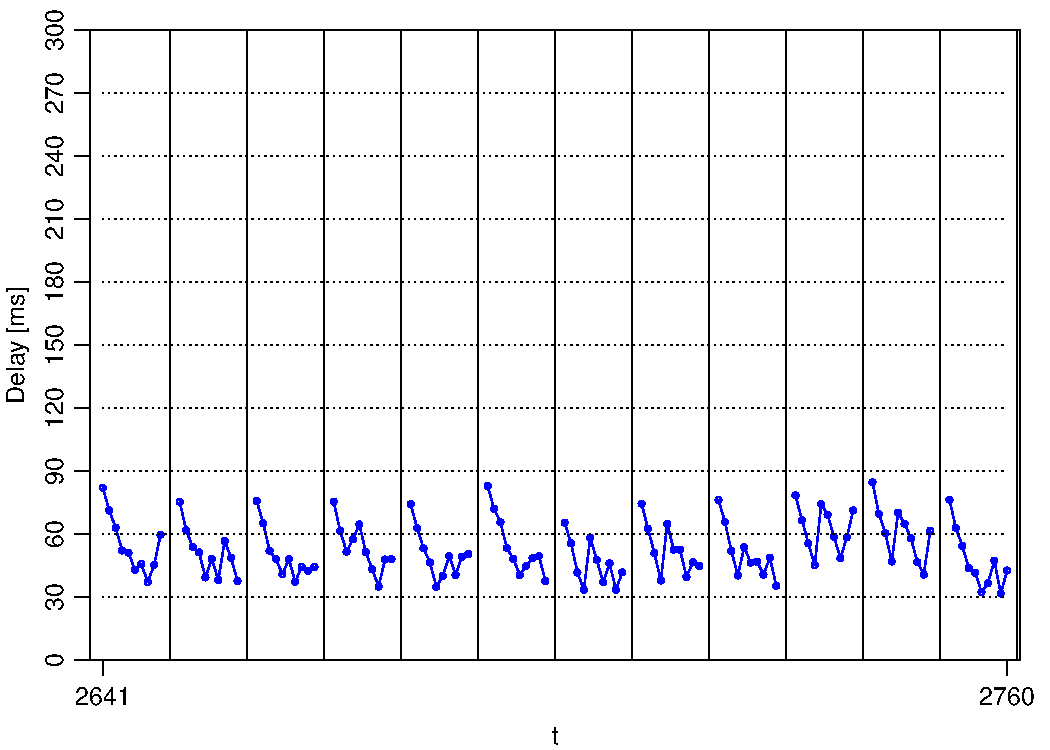
\includegraphics[width=0.33\hsize]{22-23.pdf}
}~
\subfigure[$23 \sim 24$ 分後]{
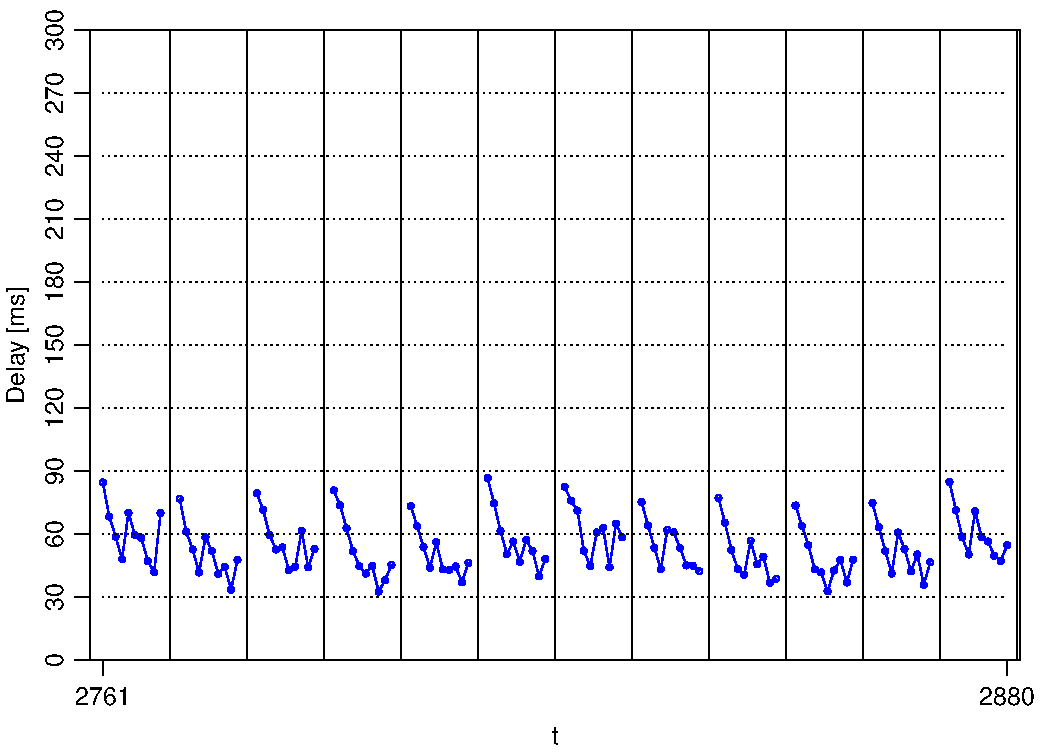
\includegraphics[width=0.33\hsize]{23-24.pdf}
}\\

\subfigure[$24 \sim 25$ 分後]{
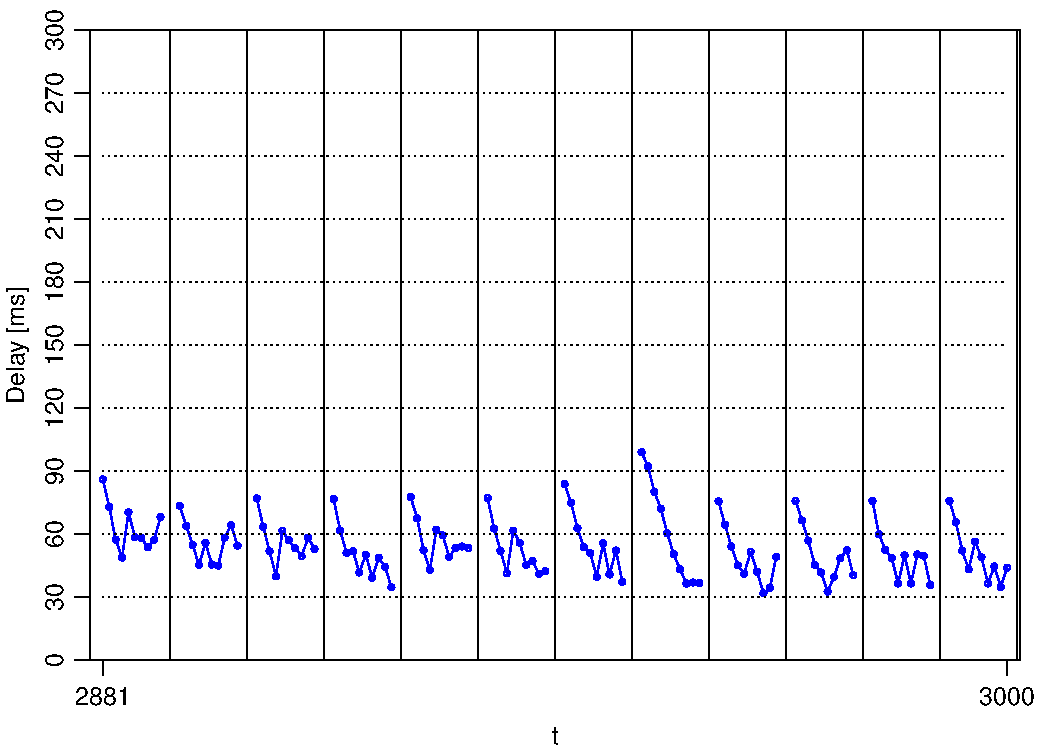
\includegraphics[width=0.33\hsize]{24-25.pdf}
}~
\subfigure[$25 \sim 26$ 分後]{
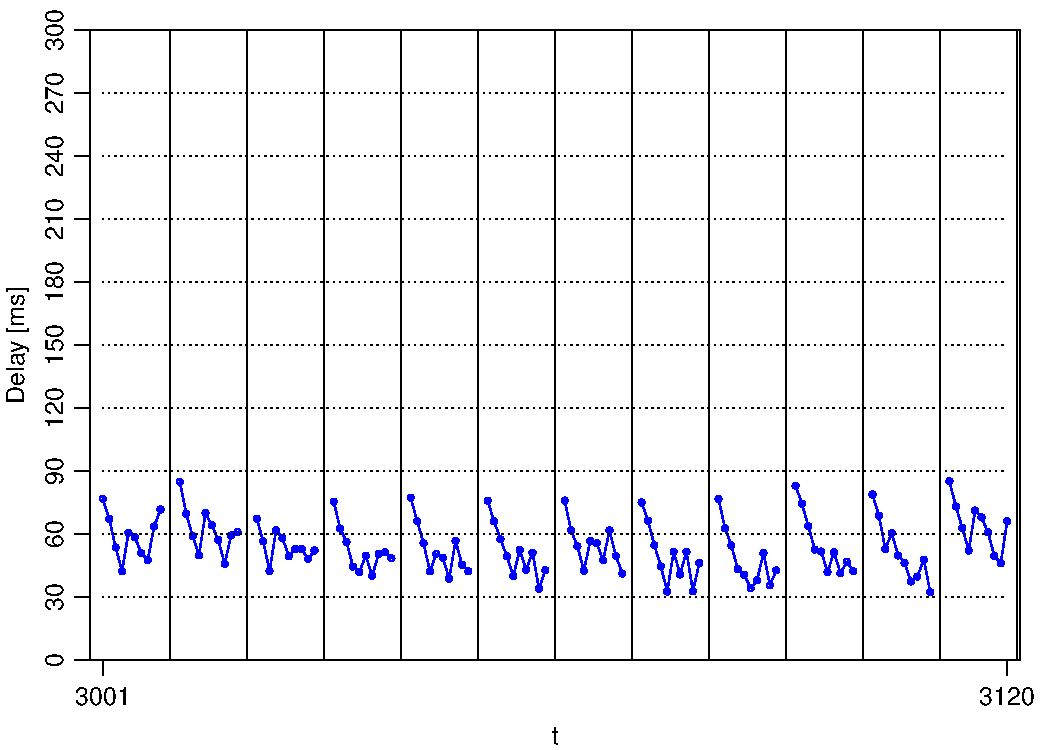
\includegraphics[width=0.33\hsize]{25-26.pdf}
}~
\subfigure[$26 \sim 27$ 分後]{
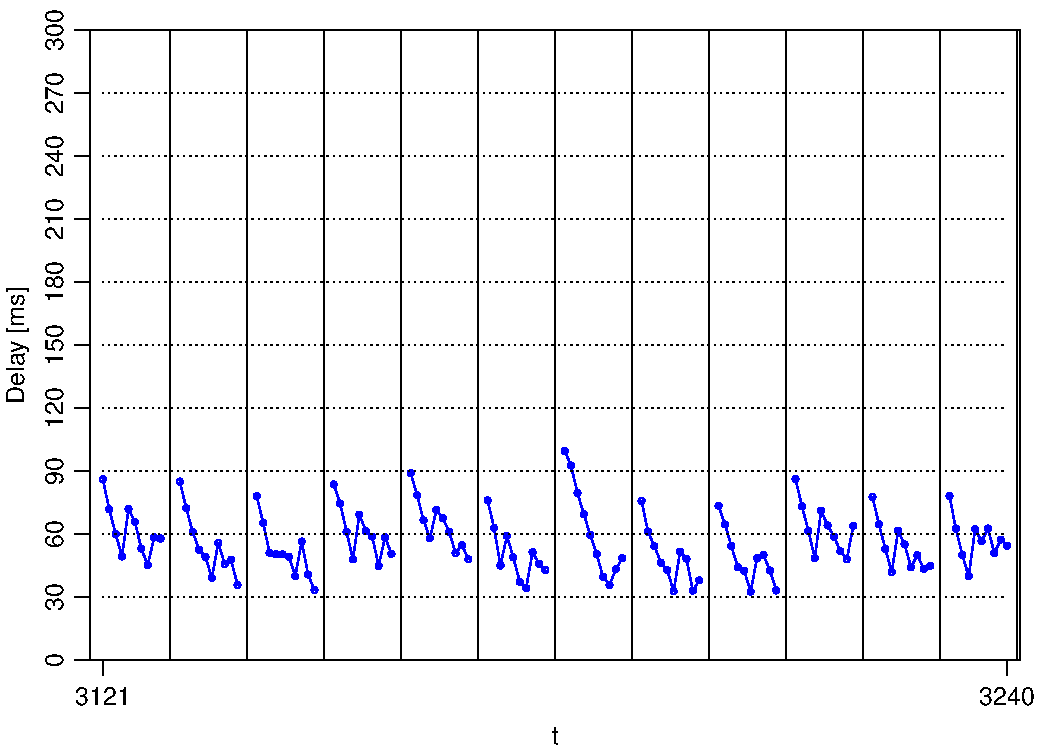
\includegraphics[width=0.33\hsize]{26-27.pdf}
}\\

\subfigure[$27 \sim 28$ 分後]{
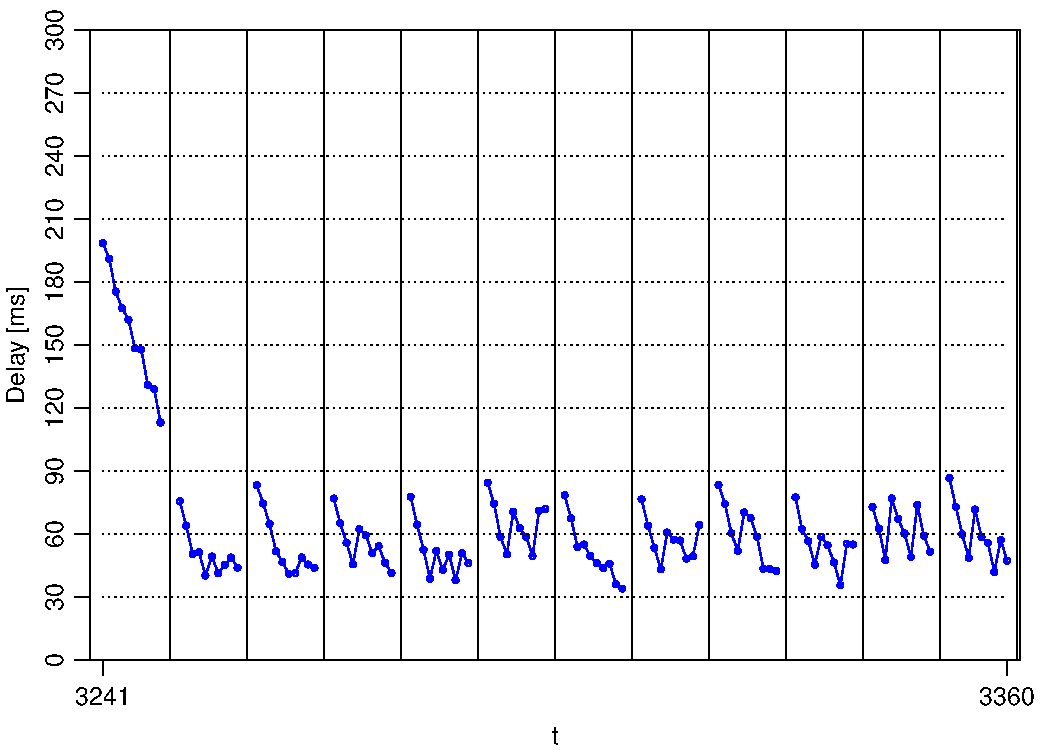
\includegraphics[width=0.33\hsize]{27-28.pdf}
}~
\subfigure[$28 \sim 29$ 分後]{
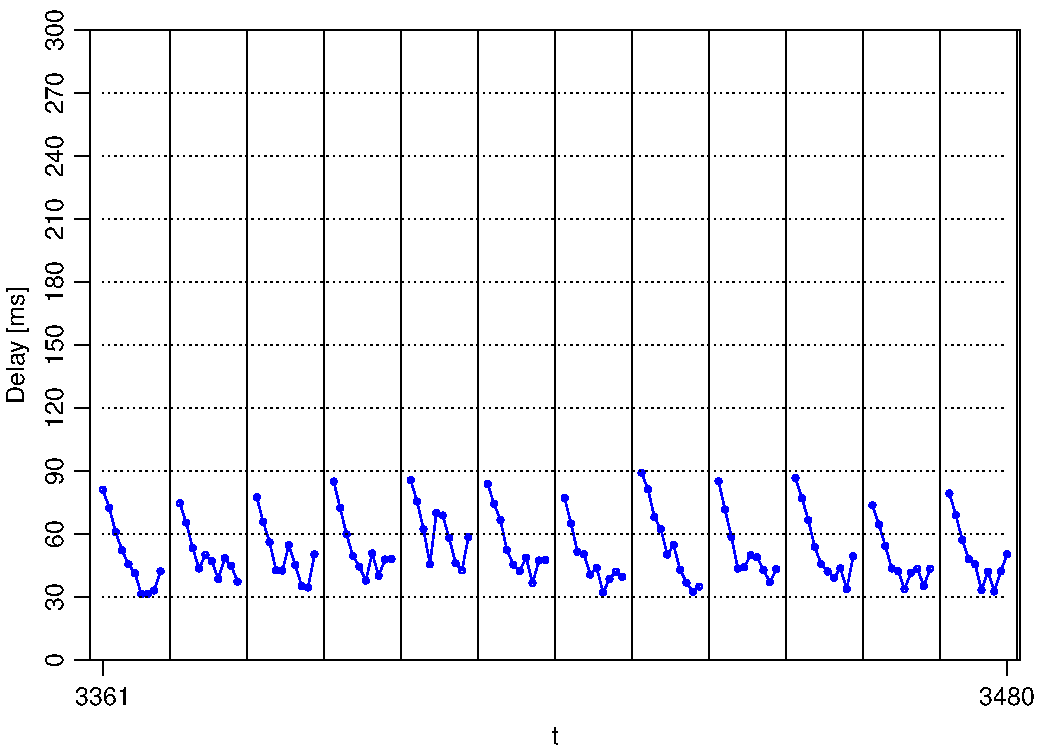
\includegraphics[width=0.33\hsize]{28-29.pdf}
}~
\subfigure[$29 \sim 30$ 分後]{
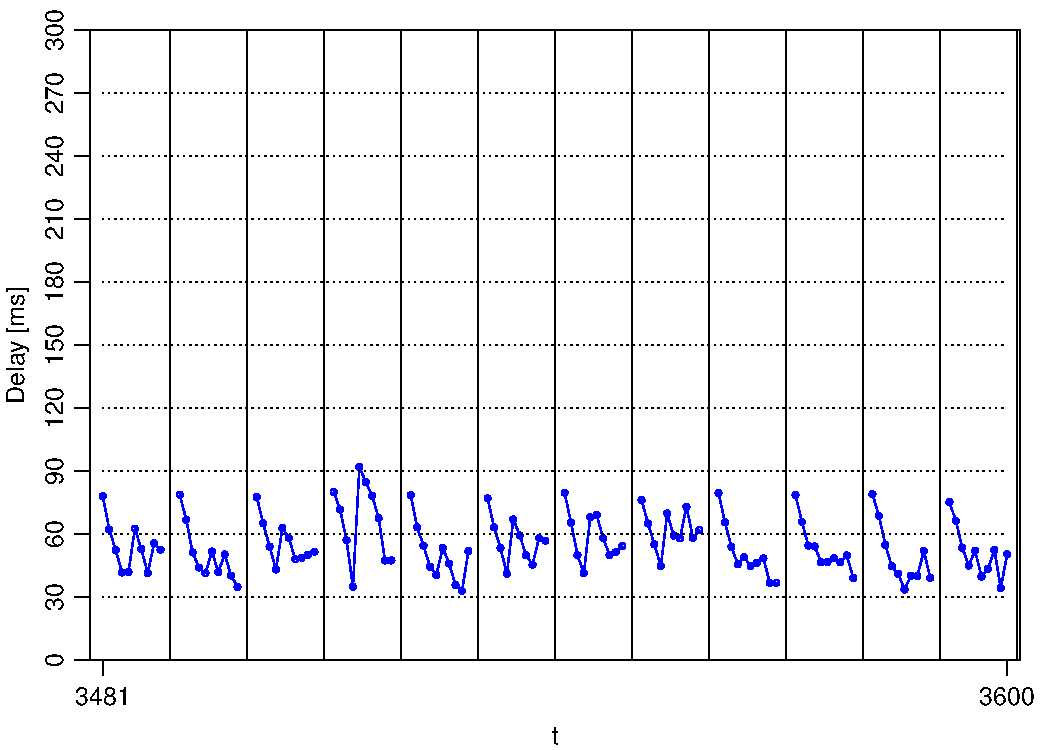
\includegraphics[width=0.33\hsize]{29-30.pdf}
}
\caption{10 ミリ秒間隔で計 10 回の ping 実行を 5 秒毎に行った計測結果(15 分後から 30 分後まで)}
\end{center}
\end{figure}

\begin{figure}[tb]
\begin{center}
\subfigure[$30 \sim 31$ 分後]{
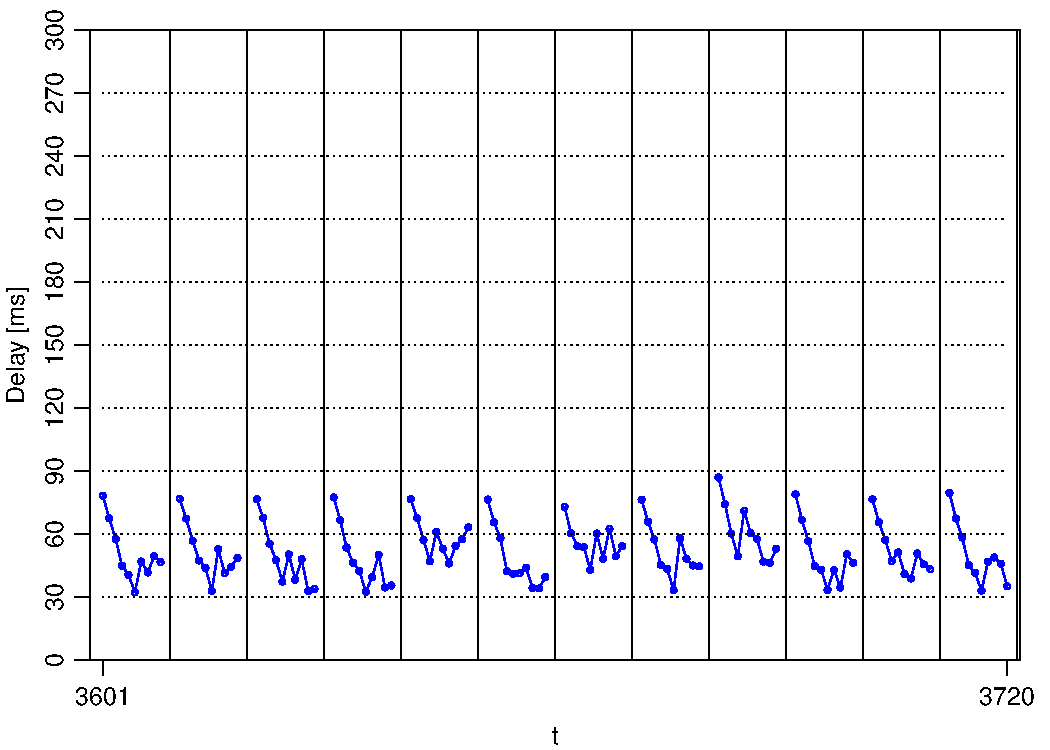
\includegraphics[width=0.33\hsize]{30-31.pdf}
}~
\subfigure[$31 \sim 32$ 分後]{
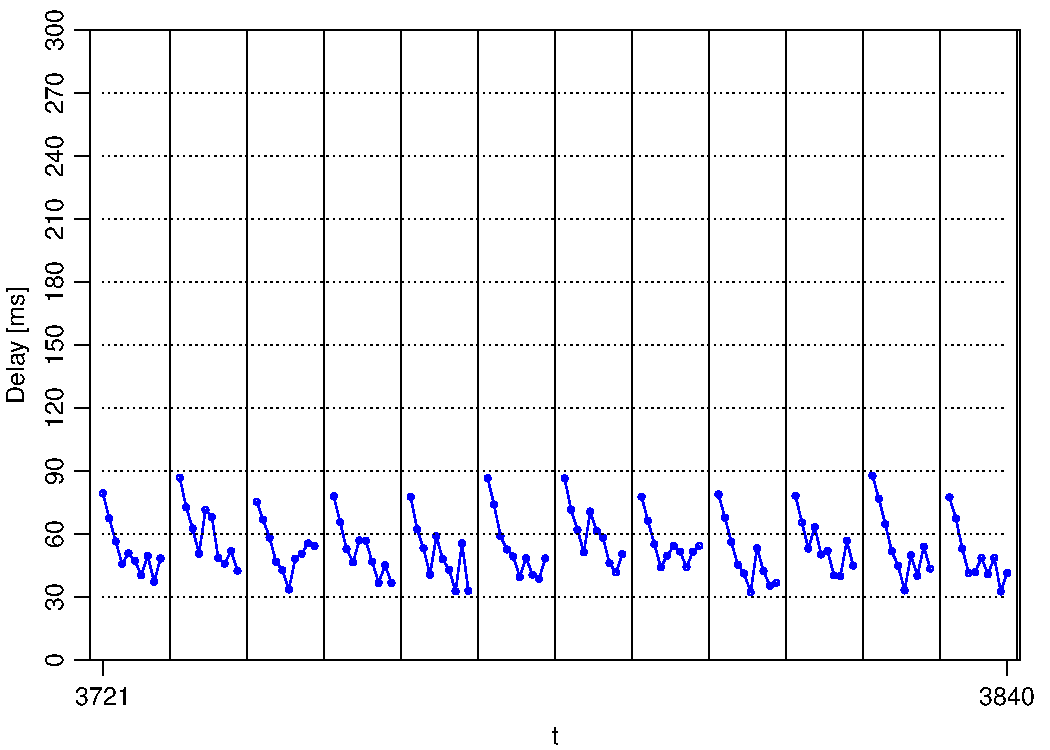
\includegraphics[width=0.33\hsize]{31-32.pdf}
}~
\subfigure[$32 \sim 33$ 分後]{
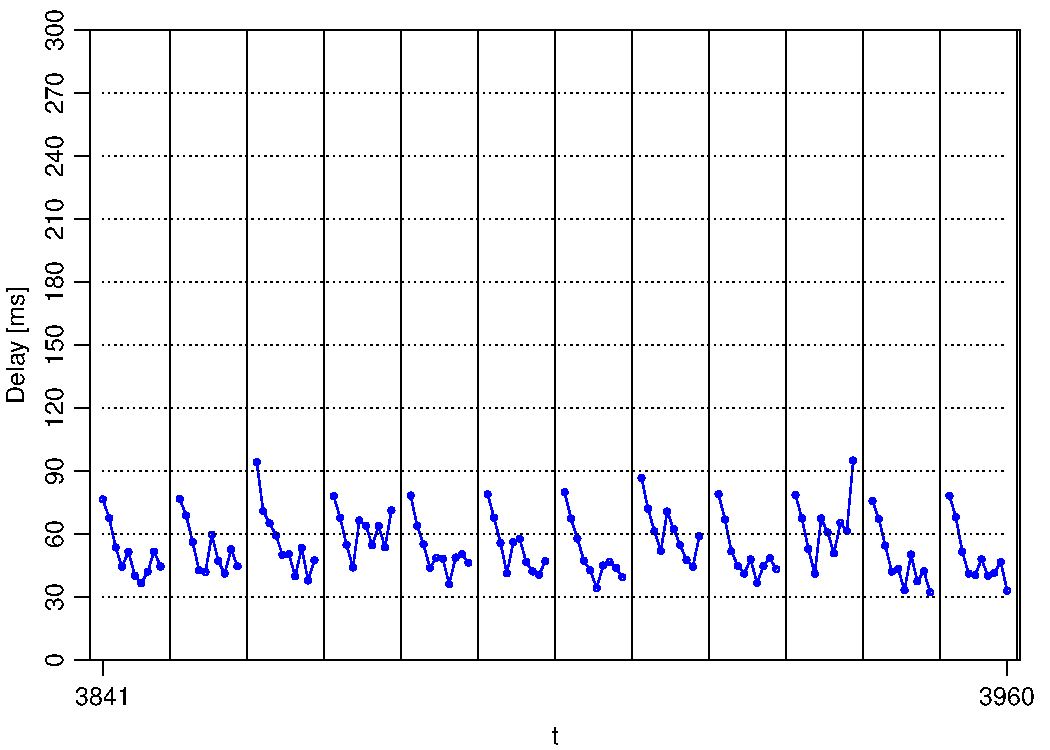
\includegraphics[width=0.33\hsize]{32-33.pdf}
}\\

\subfigure[$33 \sim 34$ 分後]{
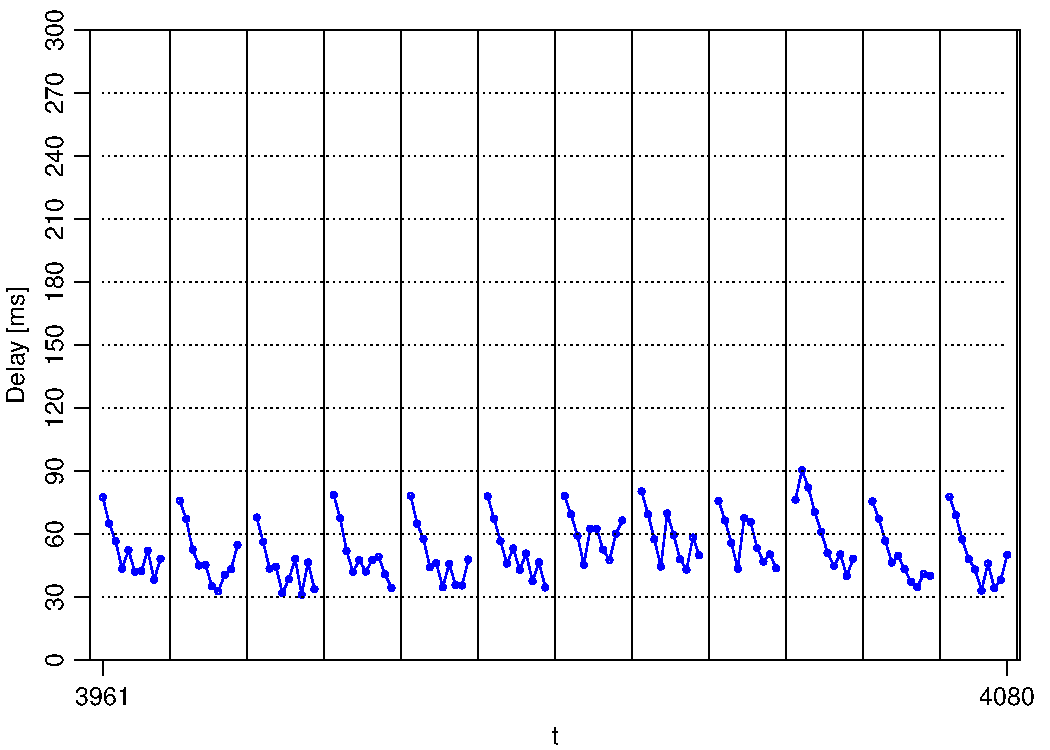
\includegraphics[width=0.33\hsize]{33-34.pdf}
}~
\subfigure[$34 \sim 35$ 分後]{
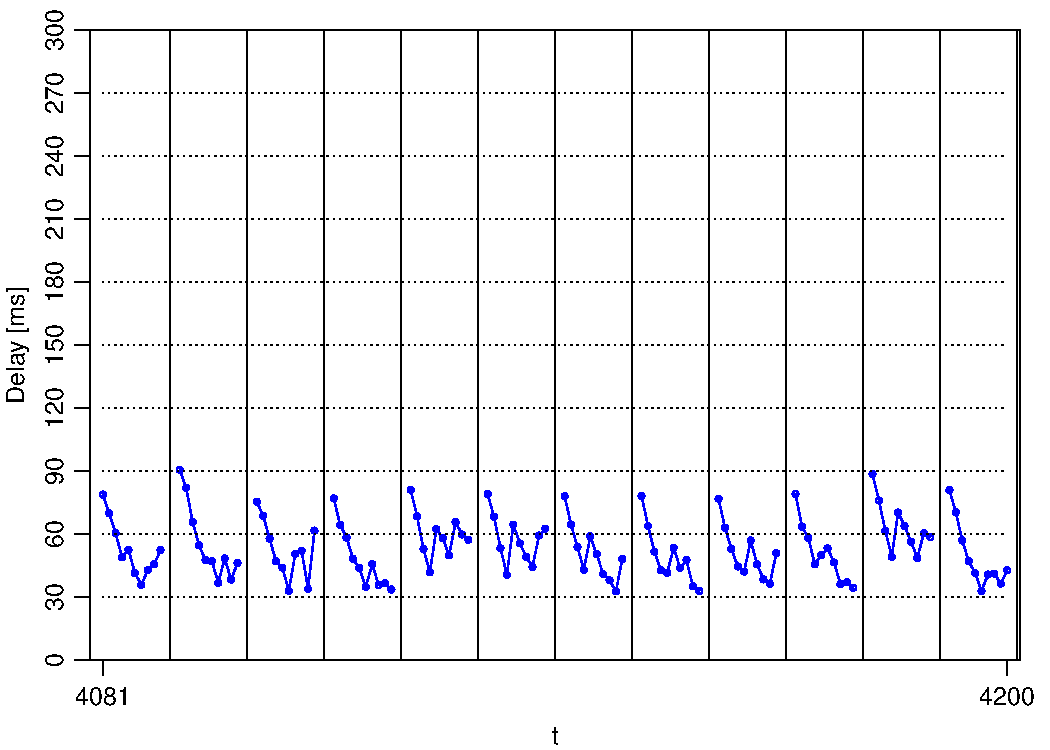
\includegraphics[width=0.33\hsize]{34-35.pdf}
}~
\subfigure[$35 \sim 36$ 分後]{
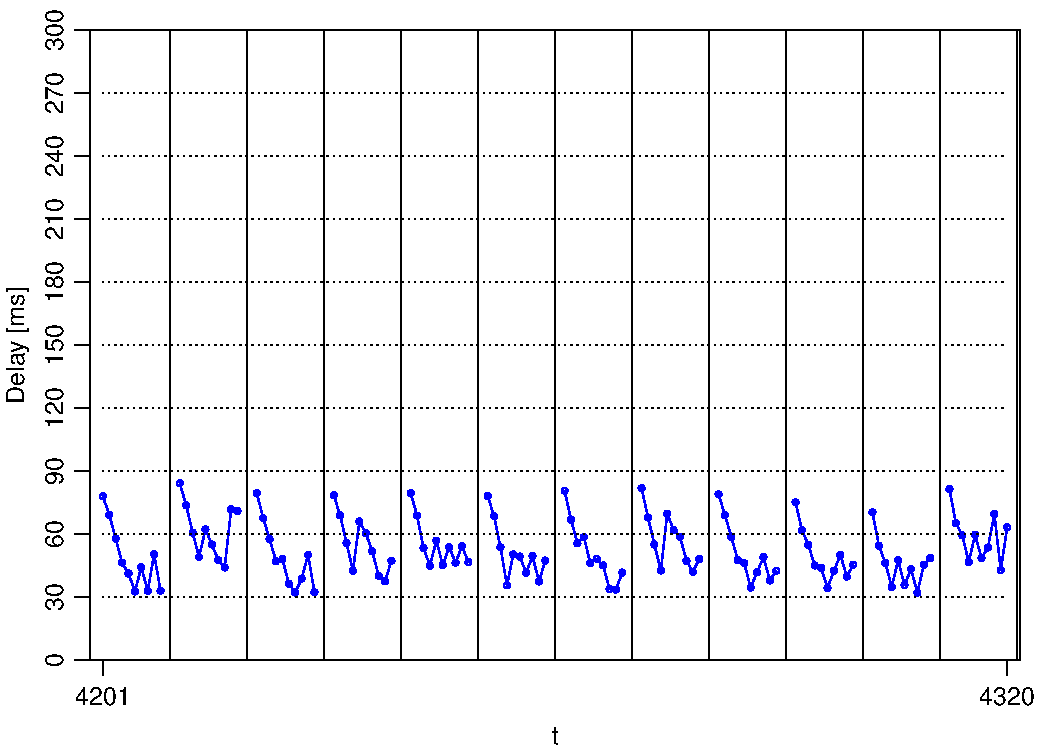
\includegraphics[width=0.33\hsize]{35-36.pdf}
}\\

\subfigure[$36 \sim 37$ 分後]{
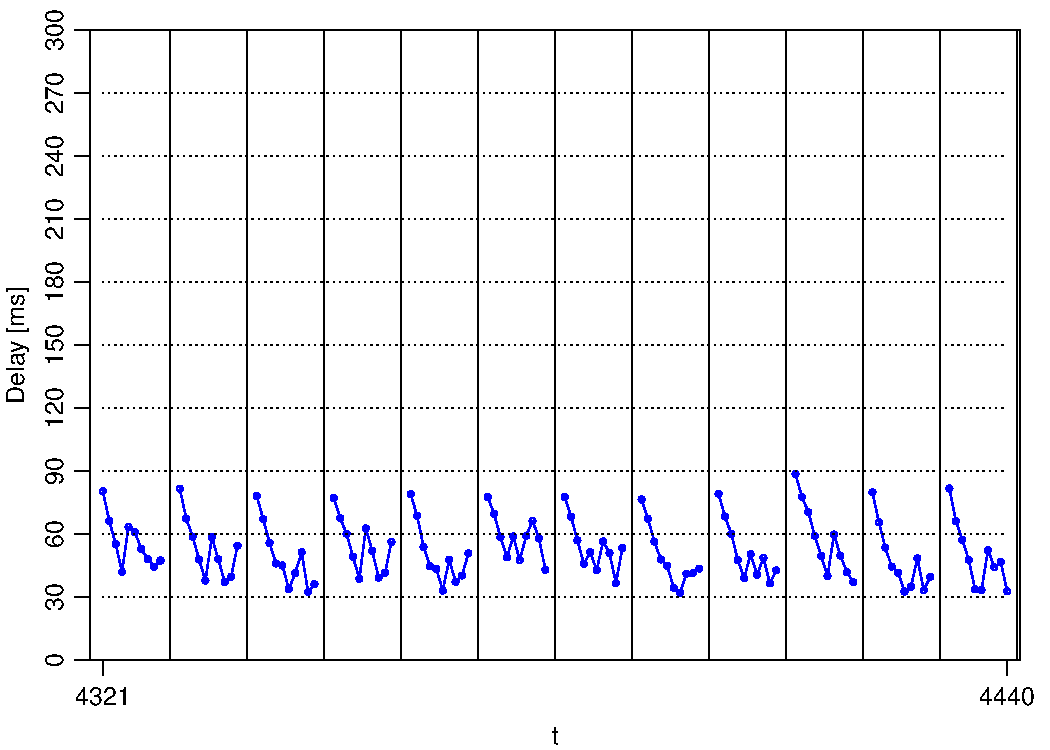
\includegraphics[width=0.33\hsize]{36-37.pdf}
}~
\subfigure[$37 \sim 38$ 分後]{
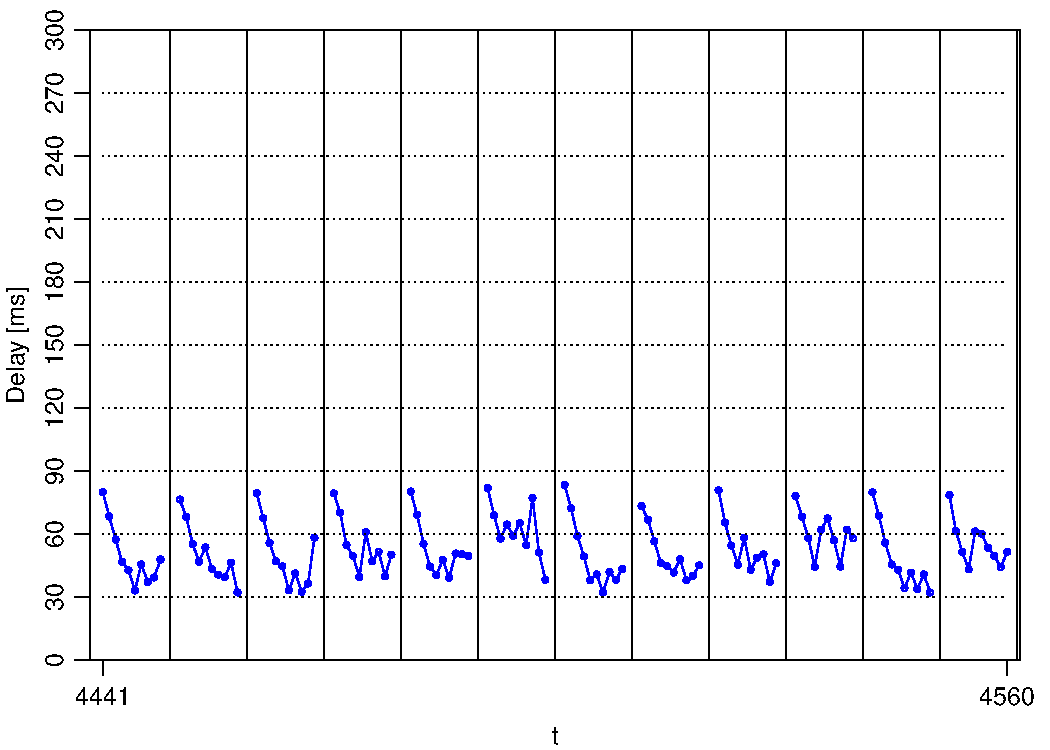
\includegraphics[width=0.33\hsize]{37-38.pdf}
}~
\subfigure[$38 \sim 39$ 分後]{
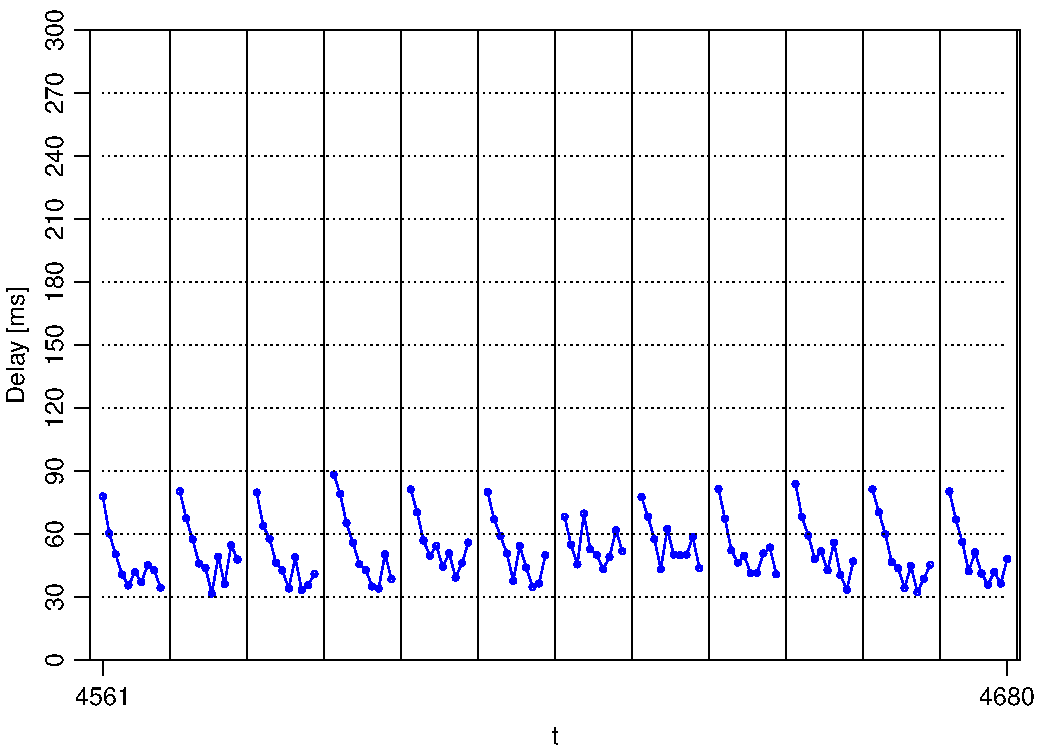
\includegraphics[width=0.33\hsize]{38-39.pdf}
}\\

\subfigure[$39 \sim 40$ 分後]{
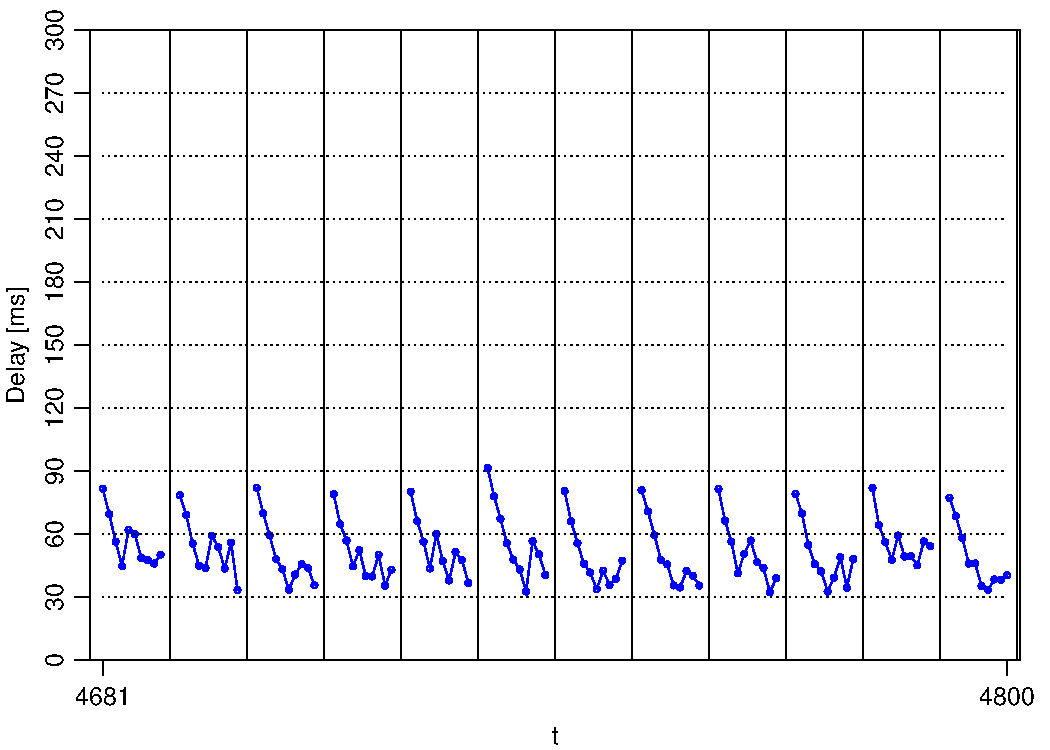
\includegraphics[width=0.33\hsize]{39-40.pdf}
}~
\subfigure[$40 \sim 41$ 分後]{
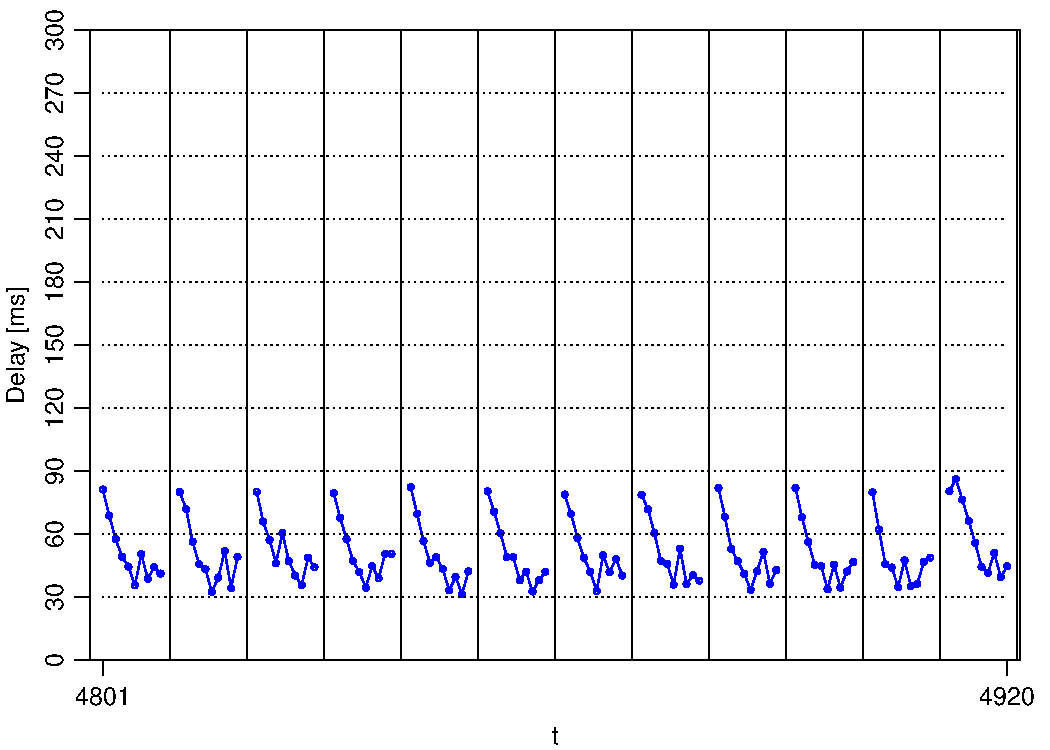
\includegraphics[width=0.33\hsize]{40-41.pdf}
}~
\subfigure[$41 \sim 42$ 分後]{
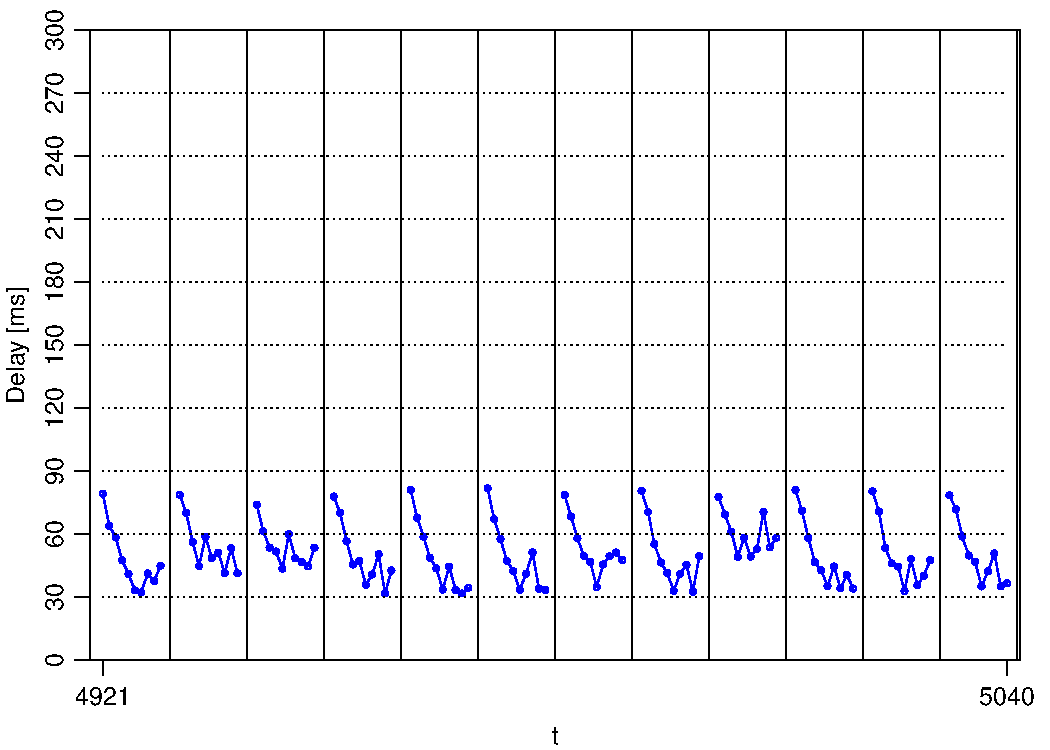
\includegraphics[width=0.33\hsize]{41-42.pdf}
}\\

\subfigure[$42 \sim 43$ 分後]{
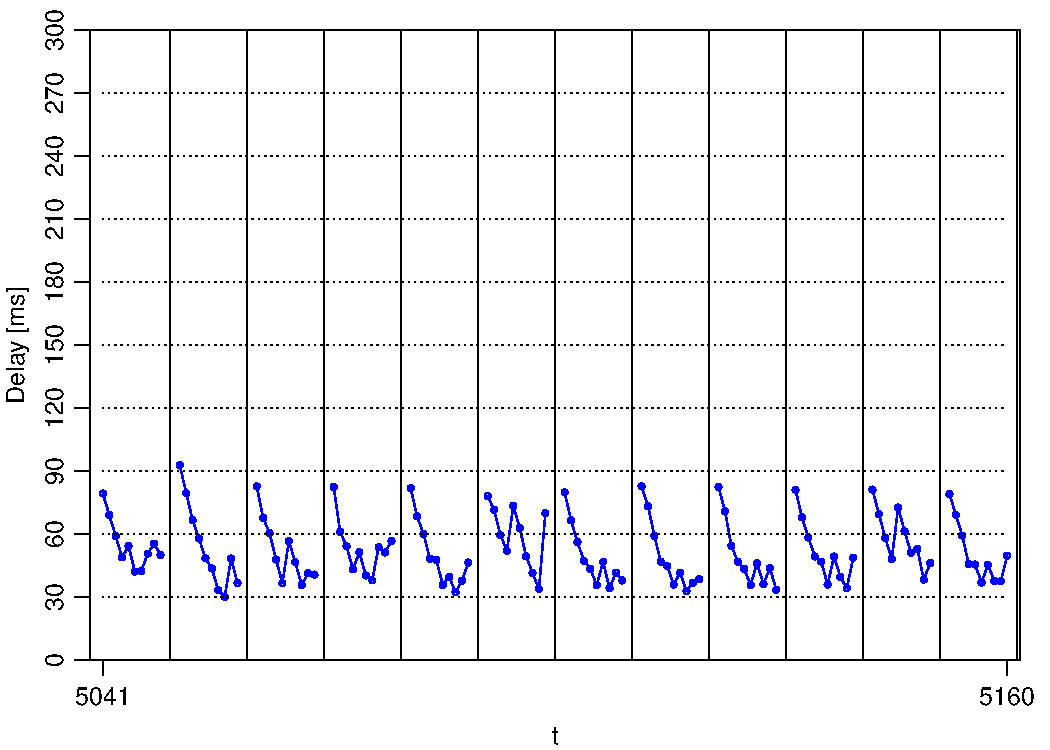
\includegraphics[width=0.33\hsize]{42-43.pdf}
}~
\subfigure[$43 \sim 44$ 分後]{
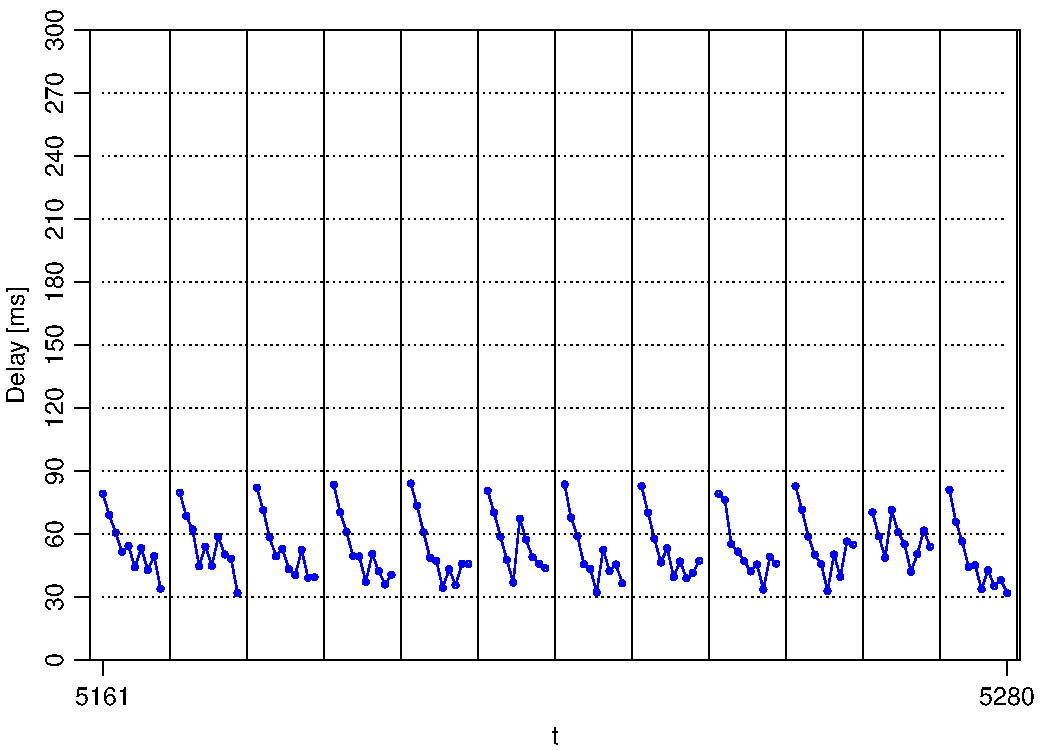
\includegraphics[width=0.33\hsize]{43-44.pdf}
}~
\subfigure[$44 \sim 45$ 分後]{
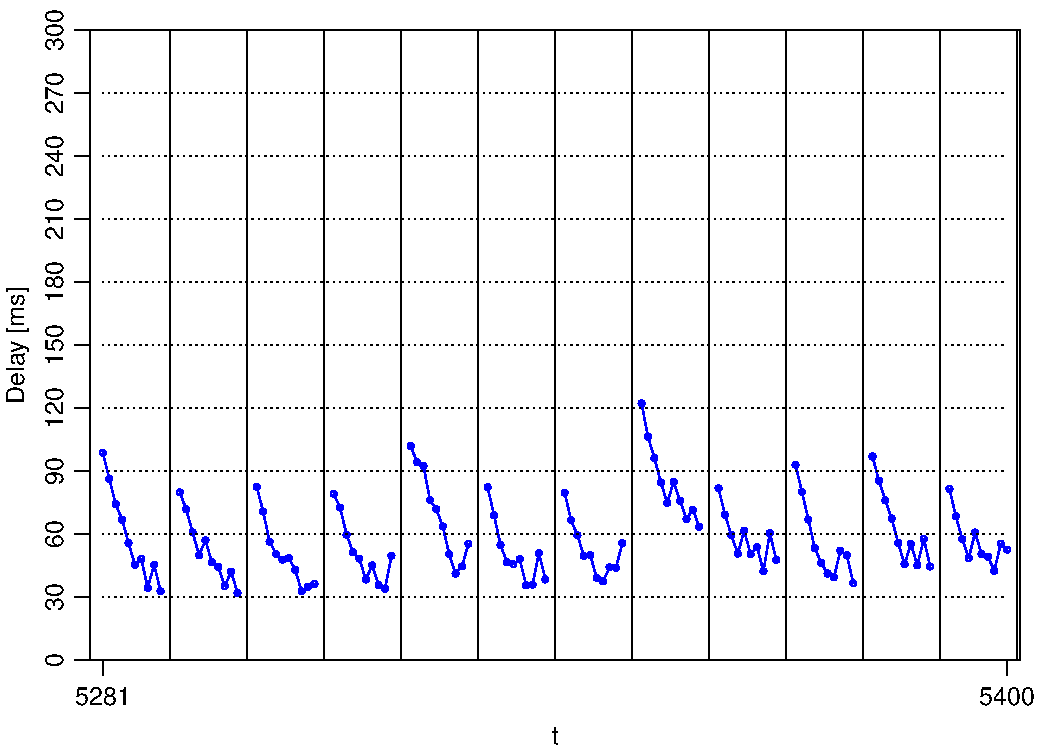
\includegraphics[width=0.33\hsize]{44-45.pdf}
}
\caption{10 ミリ秒間隔で計 10 回の ping 実行を 5 秒毎に行った計測結果(30 分後から 45 分後まで)}
\end{center}
\end{figure}

\begin{figure}[tb]
\begin{center}
\subfigure[$45 \sim 46$ 分後]{
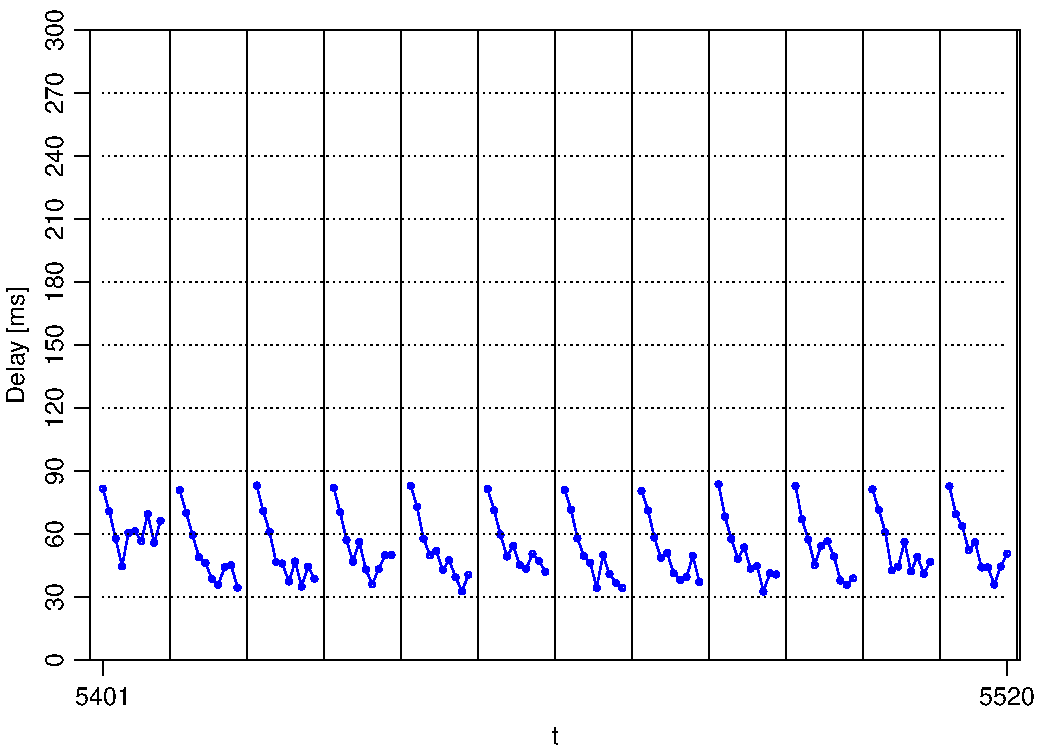
\includegraphics[width=0.33\hsize]{45-46.pdf}
}~
\subfigure[$46 \sim 47$ 分後]{
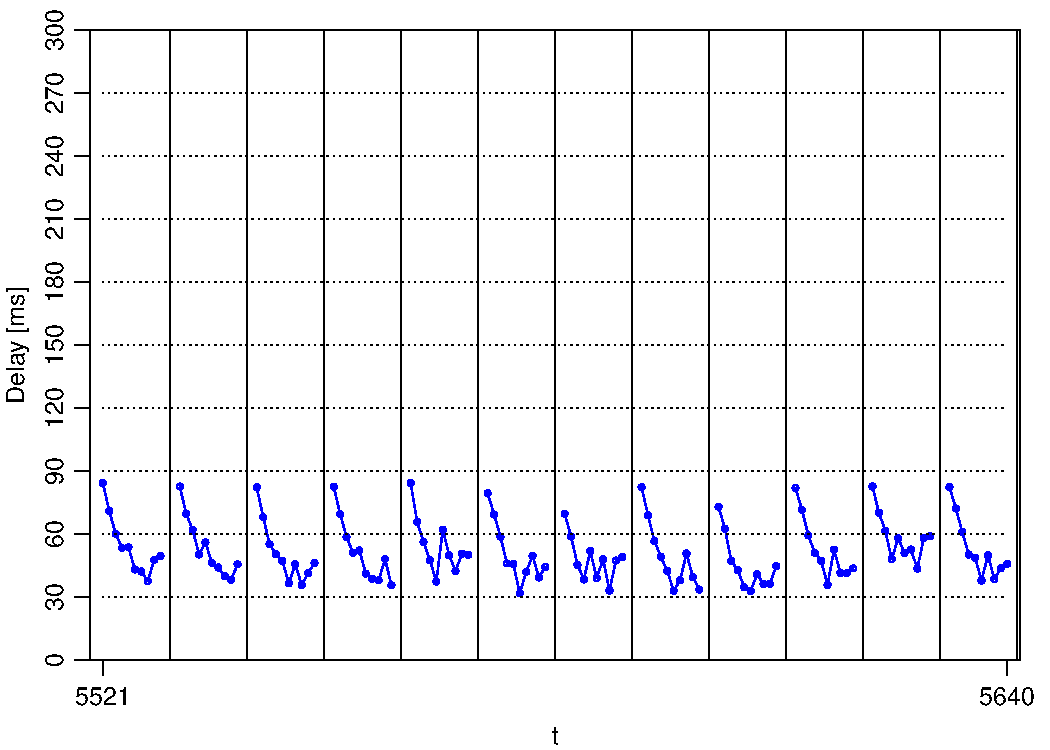
\includegraphics[width=0.33\hsize]{46-47.pdf}
}~
\subfigure[$47 \sim 48$ 分後]{
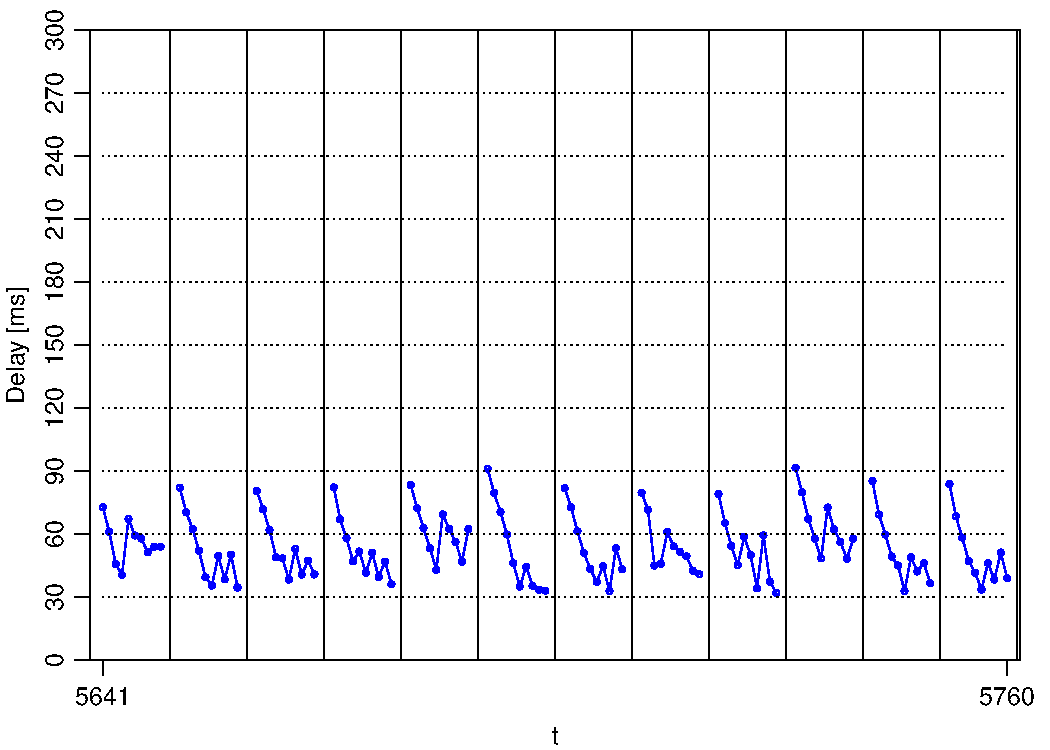
\includegraphics[width=0.33\hsize]{47-48.pdf}
}\\

\subfigure[$48 \sim 49$ 分後]{
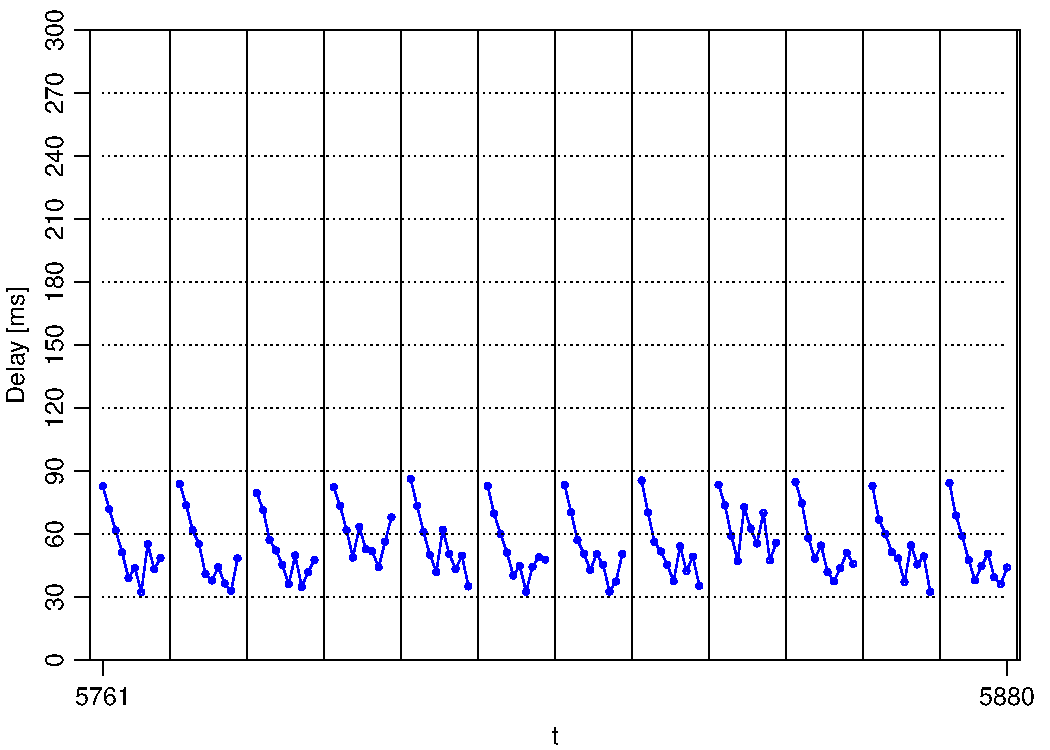
\includegraphics[width=0.33\hsize]{48-49.pdf}
}~
\subfigure[$49 \sim 50$ 分後]{
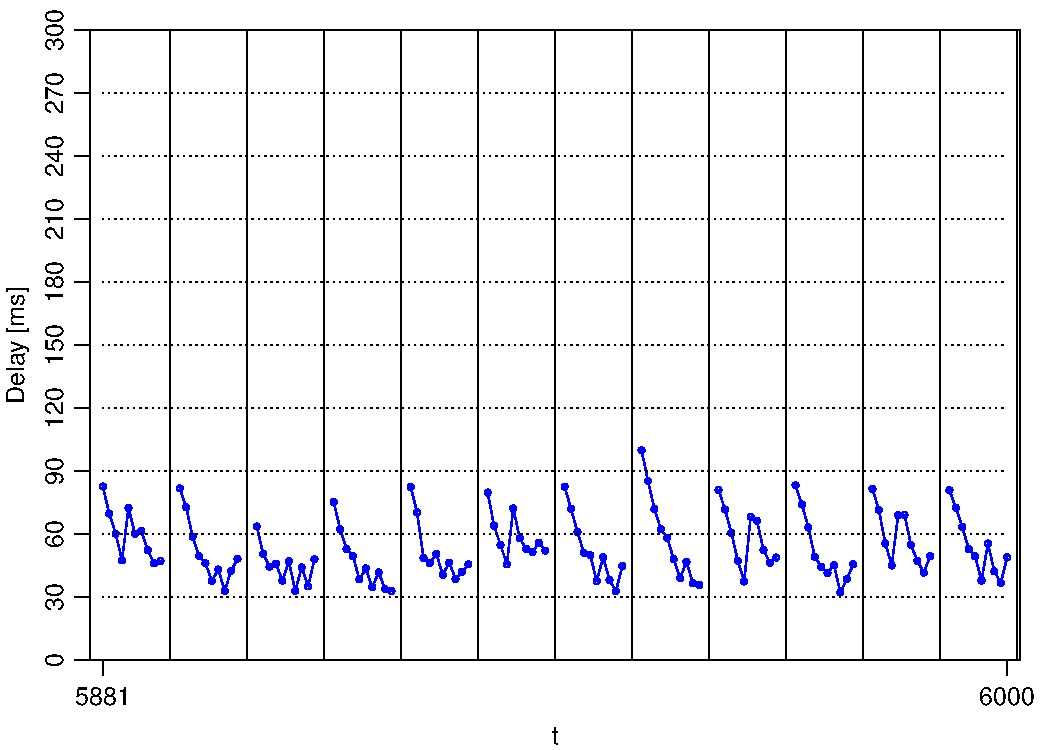
\includegraphics[width=0.33\hsize]{49-50.pdf}
}~
\subfigure[$50 \sim 51$ 分後]{
\includegraphics[width=0.33\hsize]{50-51.pdf}
}\\

\subfigure[$51 \sim 52$ 分後]{
\includegraphics[width=0.33\hsize]{51-52.pdf}
}~
\subfigure[$52 \sim 53$ 分後]{
\includegraphics[width=0.33\hsize]{52-53.pdf}
}~
\subfigure[$53 \sim 54$ 分後]{
\includegraphics[width=0.33\hsize]{53-54.pdf}
}\\

\subfigure[$54 \sim 55$ 分後]{
\includegraphics[width=0.33\hsize]{54-55.pdf}
}~
\subfigure[$55 \sim 56$ 分後]{
\includegraphics[width=0.33\hsize]{55-56.pdf}
}~
\subfigure[$56 \sim 57$ 分後]{
\includegraphics[width=0.33\hsize]{56-57.pdf}
}\\

\subfigure[$57 \sim 58$ 分後]{
\includegraphics[width=0.33\hsize]{57-58.pdf}
}~
\subfigure[$58 \sim 59$ 分後]{
\includegraphics[width=0.33\hsize]{58-59.pdf}
}~
\subfigure[$59 \sim 60$ 分後]{
\includegraphics[width=0.33\hsize]{59-60.pdf}
}
\caption{10 ミリ秒間隔で計 10 回の ping 実行を 5 秒毎に行った計測結果(45 分後から 60 分後まで)}
\label{data1-2}
\end{center}
\end{figure}

図より,組ごとに右下がりの傾向が見られ,応答遅延時間は最小応答遅延時間付近まで小さくなることが分かった.これは,後に送信される ping パケットが先に送られるパケットの影響でバッファ待ちすることなくなるからだと思われる.バッファ待ちの要因の一つとしてモバイルコアネットワークのベアラの張り直しが考えられる.この張り直しは,前の実験機器での計測において 12 秒程度の通信の途絶により発生し,5 秒では発生しないことが確認されている.SIM や OS は異なるものの,今の実験機器においても 5 秒ではベアラの張り直しは発生しないと考えた.しかしながら,図では通信間隔が最大でも 5 秒以下であるにも関わらず,10 ミリ秒間隔の最初の計測での応答遅延が大きくなっていた.したがって,今回の実験機器では,ベアラの張り直しが 5 秒程度の通信の途絶であっても発生する,もしくは,他の要因によりバッファ待ちが発生していることが考えられる.ただ,5 秒は感覚的に短くそこまで頻繁にベアラを張り直しているとは想像できないため,後者の方が可能性が高いのではないかと推測している.
\item[データ2] \\
5 秒間隔での ping による応答遅延を一日を通じて行った.横軸に時刻をとった応答遅延の結果を図 \ref{data2} に示す.また,この計測は 7 月 1 日 15 時から 7 月 2 日 15 時までのものである.
\begin{figure}[tb]
\centering
\includegraphics[width=\hsize]{plot.pdf}
\caption{ 7 月 1 日 15 時から 7 月 2 日 15 時まで(5 秒間隔)}
\label{data2}
\end{figure}
この図においても,部分的に右上がりな箇所が見て取れた.原因は現時点ではわかっていないが,5 秒という短い実行間隔であっても確認できるようだ.
\item[データ3] \\
15 秒間隔での ping による応答遅延を一日を通じて行った.現時点では,6 月 23 日(火)から 7 月 1 日(水)までの計測結果が得られている.その結果を図 \ref{data3-1} と図 \ref{data3-2} に示す.また,この計測は今後も引き続き行う.
\begin{figure}[tb]
\begin{center}
\subfigure[6 月 23 日(火)]{
\includegraphics[width=0.5\hsize]{plot-6-23.pdf}
}~
\subfigure[6 月 24 日(水)]{
\includegraphics[width=0.5\hsize]{plot-6-24.pdf}
}\\
\subfigure[6 月 25 日(木)]{
\includegraphics[width=0.5\hsize]{plot-6-25.pdf}
}~
\subfigure[6 月 26 日(金)]{
\includegraphics[width=0.5\hsize]{plot-6-26.pdf}
}\\
\subfigure[6 月 27 日(土)]{
\includegraphics[width=0.5\hsize]{plot-6-27.pdf}
}~
\subfigure[6 月 28 日(日)]{
\includegraphics[width=0.5\hsize]{plot-6-28.pdf}
}
\caption{一日を通じた計測(15 秒間隔)}
\label{data3-1}
\end{center}
\end{figure}
\begin{figure}[tb]
\begin{center}
\subfigure[6 月 29 日(月)]{
\includegraphics[width=0.5\hsize]{plot-6-29.pdf}
}~
\subfigure[6 月 30 日(火)]{
\includegraphics[width=0.5\hsize]{plot-6-30.pdf}
}\\
\subfigure[7 月 1 日(水)]{
\includegraphics[width=0.5\hsize]{plot-7-1.pdf}
}
\caption{一日を通じた計測(15 秒間隔)}
\label{data3-2}
\end{center}
\end{figure}
この結果から新たに,図 \ref{data3-1}(b) から図 \ref{data3-1}(c) までの 6 月 24 日(水)から6 月 25 日(木)にかけての大きな応答遅延の発生頻度が極端に高くなる期間や,図 \ref{data3-2}(a) の 6 月 29 日(月)のように 900 ms を超えるかなり大きな応答遅延が発生する箇所が確認された.
また,いずれの図においても部分的な右上がりの傾向が見られる.
\end{description}
\end{document}